
%% bare_conf.tex
%% V1.3
%% 2007/01/11
%% by Michael Shell
%% See:
%% http://www.michaelshell.org/
%% for current contact information.
%%
%% This is a skeleton file demonstrating the use of IEEEtran.cls
%% (requires IEEEtran.cls version 1.7 or later) with an IEEE conference paper.
%%
%% Support sites:
%% http://www.michaelshell.org/tex/ieeetran/
%% http://www.ctan.org/tex-archive/macros/latex/contrib/IEEEtran/
%% and
%% http://www.ieee.org/

%%*************************************************************************
%% Legal Notice:
%% This code is offered as-is without any warranty either expressed or
%% implied; without even the implied warranty of MERCHANTABILITY or
%% FITNESS FOR A PARTICULAR PURPOSE! 
%% User assumes all risk.
%% In no event shall IEEE or any contributor to this code be liable for
%% any damages or losses, including, but not limited to, incidental,
%% consequential, or any other damages, resulting from the use or misuse
%% of any information contained here.
%%
%% All comments are the opinions of their respective authors and are not
%% necessarily endorsed by the IEEE.
%%
%% This work is distributed under the LaTeX Project Public License (LPPL)
%% ( http://www.latex-project.org/ ) version 1.3, and may be freely used,
%% distributed and modified. A copy of the LPPL, version 1.3, is included
%% in the base LaTeX documentation of all distributions of LaTeX released
%% 2003/12/01 or later.
%% Retain all contribution notices and credits.
%% ** Modified files should be clearly indicated as such, including  **
%% ** renaming them and changing author support contact information. **
%%
%% File list of work: IEEEtran.cls, IEEEtran_HOWTO.pdf, bare_adv.tex,
%%                    bare_conf.tex, bare_jrnl.tex, bare_jrnl_compsoc.tex
%%*************************************************************************

% *** Authors should verify (and, if needed, correct) their LaTeX system  ***
% *** with the testflow diagnostic prior to trusting their LaTeX platform ***
% *** with production work. IEEE's font choices can trigger bugs that do  ***
% *** not appear when using other class files.                            ***
% The testflow support page is at:
% http://www.michaelshell.org/tex/testflow/



% Note that the a4paper option is mainly intended so that authors in
% countries using A4 can easily print to A4 and see how their papers will
% look in print - the typesetting of the document will not typically be
% affected with changes in paper size (but the bottom and side margins will).
% Use the testflow package mentioned above to verify correct handling of
% both paper sizes by the user's LaTeX system.
%
% Also note that the "draftcls" or "draftclsnofoot", not "draft", option
% should be used if it is desired that the figures are to be displayed in
% draft mode.
%
%\documentclass[conference,compsoc]{./IEEEtran}
\documentclass[10pt,conference,compsocconf]{IEEEtran}
% Add the compsoc option for Computer Society conferences.
%
% If IEEEtran.cls has not been installed into the LaTeX system files,
% manually specify the path to it like:
% \documentclass[conference]{../sty/IEEEtran}





% Some very useful LaTeX packages include:
% (uncomment the ones you want to load)


% *** MISC UTILITY PACKAGES ***
%
%\usepackage{ifpdf}
% Heiko Oberdiek's ifpdf.sty is very useful if you need conditional
% compilation based on whether the output is pdf or dvi.
% usage:
% \ifpdf
%   % pdf code
% \else
%   % dvi code
% \fi
% The latest version of ifpdf.sty can be obtained from:
% http://www.ctan.org/tex-archive/macros/latex/contrib/oberdiek/
% Also, note that IEEEtran.cls V1.7 and later provides a builtin
% \ifCLASSINFOpdf conditional that works the same way.
% When switching from latex to pdflatex and vice-versa, the compiler may
% have to be run twice to clear warning/error messages.






% *** CITATION PACKAGES ***
%
\usepackage{cite}
% cite.sty was written by Donald Arseneau
% V1.6 and later of IEEEtran pre-defines the format of the cite.sty package
% \cite{} output to follow that of IEEE. Loading the cite package will
% result in citation numbers being automatically sorted and properly
% "compressed/ranged". e.g., [1], [9], [2], [7], [5], [6] without using
% cite.sty will become [1], [2], [5]--[7], [9] using cite.sty. cite.sty's
% \cite will automatically add leading space, if needed. Use cite.sty's
% noadjust option (cite.sty V3.8 and later) if you want to turn this off.
% cite.sty is already installed on most LaTeX systems. Be sure and use
% version 4.0 (2003-05-27) and later if using hyperref.sty. cite.sty does
% not currently provide for hyperlinked citations.
% The latest version can be obtained at:
% http://www.ctan.org/tex-archive/macros/latex/contrib/cite/
% The documentation is contained in the cite.sty file itself.






% *** GRAPHICS RELATED PACKAGES ***
%
\ifCLASSINFOpdf
  \usepackage{graphicx}
  % declare the path(s) where your graphic files are
  %\graphicspath{{../img/}}
  % and their extensions so you won't have to specify these with
  % every instance of \includegraphics
  % \DeclareGraphicsExtensions{.pdf,.jpeg,.png}
\else
  % or other class option (dvipsone, dvipdf, if not using dvips). graphicx
  % will default to the driver specified in the system graphics.cfg if no
  % driver is specified.
  % \usepackage[dvips]{graphicx}
  % declare the path(s) where your graphic files are
  % \graphicspath{{../eps/}}
  % and their extensions so you won't have to specify these with
  % every instance of \includegraphics
  % \DeclareGraphicsExtensions{.eps}
\fi
% graphicx was written by David Carlisle and Sebastian Rahtz. It is
% required if you want graphics, photos, etc. graphicx.sty is already
% installed on most LaTeX systems. The latest version and documentation can
% be obtained at: 
% http://www.ctan.org/tex-archive/macros/latex/required/graphics/
% Another good source of documentation is "Using Imported Graphics in
% LaTeX2e" by Keith Reckdahl which can be found as epslatex.ps or
% epslatex.pdf at: http://www.ctan.org/tex-archive/info/
%
% latex, and pdflatex in dvi mode, support graphics in encapsulated
% postscript (.eps) format. pdflatex in pdf mode supports graphics
% in .pdf, .jpeg, .png and .mps (metapost) formats. Users should ensure
% that all non-photo figures use a vector format (.eps, .pdf, .mps) and
% not a bitmapped formats (.jpeg, .png). IEEE frowns on bitmapped formats
% which can result in "jaggedy"/blurry rendering of lines and letters as
% well as large increases in file sizes.
%
% You can find documentation about the pdfTeX application at:
% http://www.tug.org/applications/pdftex





% *** MATH PACKAGES ***
%
\usepackage[cmex10]{amsmath}
% A popular package from the American Mathematical Society that provides
% many useful and powerful commands for dealing with mathematics. If using
% it, be sure to load this package with the cmex10 option to ensure that
% only type 1 fonts will utilized at all point sizes. Without this option,
% it is possible that some math symbols, particularly those within
% footnotes, will be rendered in bitmap form which will result in a
% document that can not be IEEE Xplore compliant!
%
% Also, note that the amsmath package sets \interdisplaylinepenalty to 10000
% thus preventing page breaks from occurring within multiline equations. Use:
%\interdisplaylinepenalty=2500
% after loading amsmath to restore such page breaks as IEEEtran.cls normally
% does. amsmath.sty is already installed on most LaTeX systems. The latest
% version and documentation can be obtained at:
% http://www.ctan.org/tex-archive/macros/latex/required/amslatex/math/





% *** SPECIALIZED LIST PACKAGES ***
%
%\usepackage{algorithmic}
% algorithmic.sty was written by Peter Williams and Rogerio Brito.
% This package provides an algorithmic environment fo describing algorithms.
% You can use the algorithmic environment in-text or within a figure
% environment to provide for a floating algorithm. Do NOT use the algorithm
% floating environment provided by algorithm.sty (by the same authors) or
% algorithm2e.sty (by Christophe Fiorio) as IEEE does not use dedicated
% algorithm float types and packages that provide these will not provide
% correct IEEE style captions. The latest version and documentation of
% algorithmic.sty can be obtained at:
% http://www.ctan.org/tex-archive/macros/latex/contrib/algorithms/
% There is also a support site at:
% http://algorithms.berlios.de/index.html
% Also of interest may be the (relatively newer and more customizable)
% algorithmicx.sty package by Szasz Janos:
% http://www.ctan.org/tex-archive/macros/latex/contrib/algorithmicx/




% *** ALIGNMENT PACKAGES ***
%
\usepackage{array}
% Frank Mittelbach's and David Carlisle's array.sty patches and improves
% the standard LaTeX2e array and tabular environments to provide better
% appearance and additional user controls. As the default LaTeX2e table
% generation code is lacking to the point of almost being broken with
% respect to the quality of the end results, all users are strongly
% advised to use an enhanced (at the very least that provided by array.sty)
% set of table tools. array.sty is already installed on most systems. The
% latest version and documentation can be obtained at:
% http://www.ctan.org/tex-archive/macros/latex/required/tools/


%\usepackage{mdwmath}
\usepackage{mdwtab}
% Also highly recommended is Mark Wooding's extremely powerful MDW tools,
% especially mdwmath.sty and mdwtab.sty which are used to format equations
% and tables, respectively. The MDWtools set is already installed on most
% LaTeX systems. The lastest version and documentation is available at:
% http://www.ctan.org/tex-archive/macros/latex/contrib/mdwtools/


% IEEEtran contains the IEEEeqnarray family of commands that can be used to
% generate multiline equations as well as matrices, tables, etc., of high
% quality.


%\usepackage{eqparbox}
% Also of notable interest is Scott Pakin's eqparbox package for creating
% (automatically sized) equal width boxes - aka "natural width parboxes".
% Available at:
% http://www.ctan.org/tex-archive/macros/latex/contrib/eqparbox/





% *** SUBFIGURE PACKAGES ***
%\usepackage[tight,footnotesize]{subfigure}
% subfigure.sty was written by Steven Douglas Cochran. This package makes it
% easy to put subfigures in your figures. e.g., "Figure 1a and 1b". For IEEE
% work, it is a good idea to load it with the tight package option to reduce
% the amount of white space around the subfigures. subfigure.sty is already
% installed on most LaTeX systems. The latest version and documentation can
% be obtained at:
% http://www.ctan.org/tex-archive/obsolete/macros/latex/contrib/subfigure/
% subfigure.sty has been superceeded by subfig.sty.



%\usepackage[caption=false]{caption}
%\usepackage[font=footnotesize]{subfig}
% subfig.sty, also written by Steven Douglas Cochran, is the modern
% replacement for subfigure.sty. However, subfig.sty requires and
% automatically loads Axel Sommerfeldt's caption.sty which will override
% IEEEtran.cls handling of captions and this will result in nonIEEE style
% figure/table captions. To prevent this problem, be sure and preload
% caption.sty with its "caption=false" package option. This is will preserve
% IEEEtran.cls handing of captions. Version 1.3 (2005/06/28) and later 
% (recommended due to many improvements over 1.2) of subfig.sty supports
% the caption=false option directly:
\usepackage[caption=false,font=footnotesize]{subfig}
%
% The latest version and documentation can be obtained at:
% http://www.ctan.org/tex-archive/macros/latex/contrib/subfig/
% The latest version and documentation of caption.sty can be obtained at:
% http://www.ctan.org/tex-archive/macros/latex/contrib/caption/




% *** FLOAT PACKAGES ***
%
\usepackage{fixltx2e}
% fixltx2e, the successor to the earlier fix2col.sty, was written by
% Frank Mittelbach and David Carlisle. This package corrects a few problems
% in the LaTeX2e kernel, the most notable of which is that in current
% LaTeX2e releases, the ordering of single and double column floats is not
% guaranteed to be preserved. Thus, an unpatched LaTeX2e can allow a
% single column figure to be placed prior to an earlier double column
% figure. The latest version and documentation can be found at:
% http://www.ctan.org/tex-archive/macros/latex/base/



%\usepackage{stfloats}
% stfloats.sty was written by Sigitas Tolusis. This package gives LaTeX2e
% the ability to do double column floats at the bottom of the page as well
% as the top. (e.g., "\begin{figure*}[!b]" is not normally possible in
% LaTeX2e). It also provides a command:
%\fnbelowfloat
% to enable the placement of footnotes below bottom floats (the standard
% LaTeX2e kernel puts them above bottom floats). This is an invasive package
% which rewrites many portions of the LaTeX2e float routines. It may not work
% with other packages that modify the LaTeX2e float routines. The latest
% version and documentation can be obtained at:
% http://www.ctan.org/tex-archive/macros/latex/contrib/sttools/
% Documentation is contained in the stfloats.sty comments as well as in the
% presfull.pdf file. Do not use the stfloats baselinefloat ability as IEEE
% does not allow \baselineskip to stretch. Authors submitting work to the
% IEEE should note that IEEE rarely uses double column equations and
% that authors should try to avoid such use. Do not be tempted to use the
% cuted.sty or midfloat.sty packages (also by Sigitas Tolusis) as IEEE does
% not format its papers in such ways.





% *** PDF, URL AND HYPERLINK PACKAGES ***
%
\usepackage{url}
% url.sty was written by Donald Arseneau. It provides better support for
% handling and breaking URLs. url.sty is already installed on most LaTeX
% systems. The latest version can be obtained at:
% http://www.ctan.org/tex-archive/macros/latex/contrib/misc/
% Read the url.sty source comments for usage information. Basically,
% \url{my_url_here}.





% *** Do not adjust lengths that control margins, column widths, etc. ***
% *** Do not use packages that alter fonts (such as pslatex).         ***
% There should be no need to do such things with IEEEtran.cls V1.6 and later.
% (Unless specifically asked to do so by the journal or conference you plan
% to submit to, of course. )

\usepackage{tabularx,multirow,booktabs,xcolor}
%\usepackage{amssymb,amsmath,latexsym,mathabx,wasysym,stmaryrd}
%\usepackage[brazil]{babel}
\usepackage[utf8]{inputenc} 


% correct bad hyphenation here
\hyphenation{op-tical net-works semi-conduc-tor}


\begin{document}
%
% paper title
% can use linebreaks \\ within to get better formatting as desired
\title{Performance Inference: A Novel Approach for Planning the Capacity of IaaS Cloud Applications}


% author names and affiliations
% use a multiple column layout for up to three different
% affiliations
\author{\IEEEauthorblockN{Marcelo Gon\c{c}alves, Matheus Cunha, Nabor C. Mendon\c{c}a, Am\'erico Sampaio}
\IEEEauthorblockA{Programa de P\'os-Gradua\c{c}\~ao em Inform\'atica Aplicada (PPGIA)\\
Universidade de Fortaleza (UNIFOR)\\
Fortaleza, CE, Brazil\\
Email: \{marcelocg,mathcunha\}@gmail.com, \{nabor,americo.sampaio\}@unifor.br}}
%\author{\IEEEauthorblockN{Michael Shell}
%\IEEEauthorblockA{School of Electrical and\\Computer Engineering\\
%Georgia Institute of Technology\\
%Atlanta, Georgia 30332--0250\\
%Email: http://www.michaelshell.org/contact.html}
%\and
%\IEEEauthorblockN{Homer Simpson}
%\IEEEauthorblockA{Twentieth Century Fox\\
%Springfield, USA\\
%Email: homer@thesimpsons.com}
%\and
%\IEEEauthorblockN{James Kirk\\ and Montgomery Scott}
%\IEEEauthorblockA{Starfleet Academy\\
%San Francisco, California 96678-2391\\
%Telephone: (800) 555--1212\\
%Fax: (888) 555--1212}}

% conference papers do not typically use \thanks and this command
% is locked out in conference mode. If really needed, such as for
% the acknowledgment of grants, issue a \IEEEoverridecommandlockouts
% after \documentclass

% for over three affiliations, or if they all won't fit within the width
% of the page, use this alternative format:
% 
%\author{\IEEEauthorblockN{Michael Shell\IEEEauthorrefmark{1},
%Homer Simpson\IEEEauthorrefmark{2},
%James Kirk\IEEEauthorrefmark{3}, 
%Montgomery Scott\IEEEauthorrefmark{3} and
%Eldon Tyrell\IEEEauthorrefmark{4}}
%\IEEEauthorblockA{\IEEEauthorrefmark{1}School of Electrical and Computer Engineering\\
%Georgia Institute of Technology,
%Atlanta, Georgia 30332--0250\\ Email: see http://www.michaelshell.org/contact.html}
%\IEEEauthorblockA{\IEEEauthorrefmark{2}Twentieth Century Fox, Springfield, USA\\
%Email: homer@thesimpsons.com}
%\IEEEauthorblockA{\IEEEauthorrefmark{3}Starfleet Academy, San Francisco, California 96678-2391\\
%Telephone: (800) 555--1212, Fax: (888) 555--1212}
%\IEEEauthorblockA{\IEEEauthorrefmark{4}Tyrell Inc., 123 Replicant Street, Los Angeles, California 90210--4321}}




% use for special paper notices
%\IEEEspecialpapernotice{(Invited Paper)}




% make the title area
\maketitle


\begin{abstract}
%\boldmath

This work proposes a novel approach to support application capacity planning in infrastructure-as-a-service (IaaS) clouds. The proposed approach relies on the assumption that there exists a capacity relation between different resource configurations offered by a given IaaS cloud provider, enabling one to predict (or ``infer''), with high accuracy, an application's expected performance for certain resource configurations and workloads, based upon its observed performance for other resource configurations and workloads in that same provider. Preliminary empirical results, obtained from evaluating the performance of a well-known blogging application (WordPress) in a public cloud provider (Amazon EC2), show that the proposed approach can significantly reduce (over 85\%) the total number of application deployment options that need to be effectively tested in the cloud.

\end{abstract}
% IEEEtran.cls defaults to using nonbold math in the Abstract.
% This preserves the distinction between vectors and scalars. However,
% if the conference you are submitting to favors bold math in the abstract,
% then you can use LaTeX's standard command \boldmath at the very start
% of the abstract to achieve this. Many IEEE journals/conferences frown on
% math in the abstract anyway.
"% no keywords




% For peer review papers, you can put extra information on the cover
% page as needed:
% \ifCLASSOPTIONpeerreview
% \begin{center} \bfseries EDICS Category: 3-BBND \end{center}
% \fi
%
% For peerreview papers, this IEEEtran command inserts a page break and
% creates the second title. It will be ignored for other modes.
%\IEEEpeerreviewmaketitle



\section{Introduction}\label{sec:intro}

%A computação em nuvem é um paradigma computacional que está transformando a forma de desenvolver e gerenciar aplicações e serviços de Tecnologia da Informação \cite{Murugesan2014}. Diversas organizações passaram a adotar este paradigma atraídas pelo seu modelo de negócios onde recursos computacionais (ex.: computação, armazenamento e transferência de dados) podem ser consumidos, sob-demanda, como um serviço e pagos de acordo com o consumo efetuado. 

Um dos principais desafios enfrentados pelos usuários de nuvens que oferecem infraestrutura-como-serviço (IaaS) é planejar adequadamente a capacidade dos recursos da nuvem necessários para atender as demandas específicas de suas aplicações \cite{Menasce2009}.  Parte desse desafio envolve tentar descobrir a melhor maneira de implantar a aplicação na nuvem, considerando os vários tipos de recursos (em particular, máquinas virtuais) oferecidos pelo provedor, sob a perspectiva de diferentes requisitos e critérios de qualidade \cite{GoncalvesJunior2015}.  

Em geral, provedores de nuvens IaaS cobram seus usuários em função do tempo de utilização dos recursos solicitados, cujos preços variam conforme a capacidade (normalmente medida por características técnicas como quantidade de núcleos de processamento, tamanho de memória e espaço de armazenamento) de cada recurso. Dessa forma, para calcular o custo de operação de uma aplicação na nuvem, é preciso estimar ou medir como a aplicação responderá a diferentes níveis de demanda, em termos de indicadores de desempenho como tempo de resposta ou vazão, quando executada sob diferentes configurações e perfis de máquinas virtuais. Na prática, isso significa que cabe ao usuário da nuvem identificar, dentre as possíveis configurações de máquinas virtuais ofertadas por um ou mais provedores de nuvem, aquelas de menor custo capazes de executar a aplicação mantendo-se níveis satisfatórios para os indicadores de desempenho.

% ... Somem-se a isso as inúmeras possibilidades de implantação da aplicação considerando tanto estratégias de escalabilidade vertical (variando-se a quantidade de recursos de cada máquina) quanto horizontal (variando-se a quantidade de máquinas em uma ou mais camadas da aplicação, como dados, apresentação e negócio), chega-se a um conjunto bastante amplo de cenários de implantação a serem investigados. 

%Outro desafio ao planejamento de capacidade decorre da constatação de que configurações formadas por recursos com perfis similares, ainda que do mesmo provedor, podem responder de maneira diferente quando submetidas a um mesmo nível de carga de trabalho, a depender do momento em que sejam utilizadas \cite{cunha2011investigating, iosup2011performance, jayasinghe2011variations}. Independente do motivo que leve a esse comportamento de certa forma imprevisível, é preciso levar em conta nos testes de avaliação de desempenho essa variabilidade, o que pode pode ser alcançado através da repetição dos cenários de teste em horários e dias diferentes.

Um grande problema começa a se desenhar para o usuário da nuvem ao seguir essa abordagem: a fase de avaliação da 
aplicação pode atingir patamares elevados de tempo e custo, em razão das necessidades de variação da demanda, da 
arquitetura de implantação e das configurações de recursos utilizadas para hospedar 
cada camada da aplicação \cite{silva2013cloudbench}. Ainda que certos provedores IaaS ofereçam descontos ou 
pacotes de horas grátis para novos clientes, em geral esses incentivos, por estarem limitados a máquinas de pequeno porte, são 
insuficientes para suportar a carga de uma aplicação real em produção. Assim, executar uma aplicação real, tipicamente 
implantada em arquitetura de várias camadas~\cite{jayasinghe2011variations}, em máquinas virtuais de tamanho 
considerável e por longos períodos de tempo, apenas para estudar o seu comportamento, pode se traduzir em um custo 
alto que dificulte ou até mesmo inviabilize o próprio projeto de migração dessa aplicação para a nuvem~\cite{beserra2012cloudstep}. 

Vários trabalhos já foram propostos com o intuito de apoiar o planejamento da capacidade de aplicações em nuvens IaaS. Em 
linhas gerais, esses trabalhos podem ser classificados de acordo duas abordagens distintas quanto à estratégia de 
avaliação do desempenho da aplicação. Trabalhos que seguem a primeira abordagem, referenciada neste 
trabalho como \emph{abordagem preditiva}, visam estimar ou simular o desempenho esperado da aplicação para determinadas 
configurações de recursos e determinados níveis de carga, sem necessariamente
ter que implantá-la na nuvem  \cite{cloudharmony, malkowski2010cloudxplor, li2011, li2011cloudprophet, fittkau2012cdosim, jung2013cloudadvisor}. Apesar do baixo custo oferecido aos usuários, que não precisam pagar por recursos de nuvem durante a fase de avaliação, esse trabalhos têm como maior limitação a ainda baixa precisão das técnicas de predição de desempenho, particularmente daquelas baseadas em simulação~\cite{fittkau2012cdosim}. Já os trabalhos que fazem parte da segunda abordagem, aqui referenciada como \emph{abordagem empírica}, tem como objetivo medir o desempenho real da aplicação através de sua efetiva implantação na nuvem e da realização de testes de carga \cite{jayasinghe2012, silva2013cloudbench, cunha2013b, scheuner2014cloud}. Por executarem a aplicação no próprio ambiente de nuvem, esses trabalhos conseguem resultados significativamente mais precisos no que diz respeito à seleção das melhores configurações de recursos para cargas de trabalho específicas. No entanto, uma limitação importante desses trabalhos é a necessidade de se testar exaustivamente uma grande quantidade de configurações de recursos e cargas de trabalho, implicando em altos custos durante a fase de avaliação.

%As técnicas de predição de desempenho adotadas na abordagem preditiva variam conforme o trabalho, sendo as mais comuns o uso de simuladores \cite{fittkau2012cdosim} e a analogia com resultados previamente obtidos através da utilização de \emph{benchmarks} \cite{cloudharmony, malkowski2010cloudxplor}. Apesar do baixo custo oferecido aos usuários, que não precisam pagar por recursos de nuvem durante a fase de avaliação, trabalhos da abordagem preditiva têm como maior limitação uma ainda baixa precisão na sua  capacidade de prever o desempenho da aplicação alvo. Isto se deve principalmente a diferenças conceituais entre o ambiente da nuvem real e os modelos de simulação \cite{fittkau2012cdosim}, ou à ausência de \emph{benchmarks} com comportamento e perfis de carga de trabalho similares aos da aplicação alvo. Já os trabalhos que utilizam a abordagem empírica, por executarem a aplicação no próprio ambiente de nuvem, conseguem obter resultados significativamente mais precisos no que diz respeito à seleção das melhores configurações de recursos para cargas de trabalho específicas. No entanto, uma limitação importante desses trabalhos é a necessidade de se testar exaustivamente uma grande quantidade de configurações de recursos e cargas de trabalho, implicando em altos custos durante a fase de avaliação.

Visando combinar as vantagens das abordagens preditiva e empírica, este trabalho propõe uma nova maneira de apoiar os usuários de nuvens IaaS a identificarem as melhores (i.e., mais baratas) configurações de recursos capazes de satisfazer as demandas específicas de suas aplicações. A nova abordagem tem como premissa a existência de uma relação de capacidade entre diferentes configurações de recursos oferecidas por um dado provedor de nuvem, 
com a qual é possível prever (ou ``inferir''), com alta precisão, o desempenho esperado da aplicação para determinadas configurações de recursos. A predição ou inferência é realizada com base no desempenho observado da aplicação para outras configurações de recursos e cargas de trabalho no mesmo provedor. Por exemplo, se a aplicação atendeu satisfatoriamente a demanda para uma configuração de recursos de determinada capacidade sob uma determinada carga de trabalho, é muito provável que ela também vá atendê-la para outras configurações de maior capacidade sob a mesma carga de trabalho. Analogamente, se a aplicação não atendeu a demanda para uma determinada configuração de recursos sob uma determinada carga de trabalho, muito provavelmente ela também não irá atendê-la para a mesma configuração sob cargas de trabalho maiores. Através do uso de inferência, a abordagem permite avaliar uma ampla variedade de cenários de implantação da aplicação, sendo que apenas uma pequena parte desses cenários precisa de fato ser implantada e executada na nuvem. Dessa forma, a abordagem consegue obter o melhor das duas abordagens previamente citadas, produzindo resultados de alta precisão (característicos da abordagem empírica) mas com significativa redução de custo (característica da abordagem preditiva).

A próxima seção apresenta um novo processo de avaliação de capacidade para aplicações na nuvem, fundamentado no conceito de inferência de desempenho. A Seção~\ref{sec:experiments} descreve os resultados de uma avaliação preliminar do novo processo envolvendo a implantação de uma aplicação real em um provedor de nuvem IaaS público. A Seção~\ref{sec:related-work} compara o novo processo com outros trabalhos relacionados. Por fim, a Seção~\ref{sec:conclusion} oferece as conclusões e sugestões para trabalhos futuros.


\section{The Proposed Capacity Evaluation Process}\label{sec:process}

\subsection{Concepts and Terminology}

Antes de apresentarmos o processo, é necessário definirmos alguns conceitos importantes relacionados ao domínio da avaliação da capacidade de aplicações na nuvem (ver \mbox{Tabela~\ref{tab:concepts}}). A definição desses conceitos também serve para estabelecer a terminologia que será utilizada na descrição do processo, feita a seguir.

\begin{table}[t*]
\setlength{\tabcolsep}{3pt}
\centering%\scriptsize
\caption{Concepts and terminology used in the paper.}
\label{tab:concepts}
%\tabsize
%\begin{tabularx}{\linewidth}{|>{\centering}p{1.1cm}<{\centering}|X|}
\begin{tabularx}{\linewidth}{|p{1.35cm}|X|}
\hline%\hline
%\toprule
\centering Concept & \multicolumn{1}{c|}{Definition} \\
\hline
%\midrule
\emph{Aplication\newline under Test} & Um sistema computacional, possivelmente implementado em uma arquitetura multicamadas, para o qual se deseja observar o comportamento em um ambiente de computação em nuvem e ao qual estão associadas uma ou mais {\em métricas de desempenho}.
\\%[0.06cm]
\hline
\emph{Performance\newline Metric} &
Uma característica ou comportamento mensurável de forma automatizada e comparável a um {\em valor de referência}, capaz de indicar o grau de sucesso de uma execução da aplicação sob teste. É dependente do domínio da aplicação. Ex.: tempo de resposta, quadros por segundo.
\\%[0.06cm]
\hline
\emph{Reference\newline Value (SLA)} &
Um valor predefinido como minimamente aceitável  para uma métrica de desempenho após uma execução da aplicação sob teste. Este valor, também referenciado neste trabalho como SLA (\emph{Service Level Agreement}), serve como base de comparação para que se classifique a aplicação como capaz de ser executada em uma certa {\em configuração} de máquinas virtuais e sob uma certa {\em carga de trabalho}.
\\%[0.06cm]
\hline
\emph{Cloud\newline Provider} &
Uma empresa que fornece recursos computacionais como serviço cobrado financeiramente por fração de tempo de utilização. Neste trabalho, o foco será em provedores que disponibilizam recursos de infraestrutura, notadamente {\em máquinas virtuais}.
\\%[0.06cm]
\hline
\emph{VM Types} &
Classificam as máquinas virtuais fornecidas por um provedor conforme suas características técnicas (e.g., núcleos de processamento, tamanho de memória, espaço em disco), permitindo que o provedor mantenha uma linha de produtos discreta e finita.
\\%[0.06cm]
\hline
\emph{VM Category} &
Agrupam os tipos de máquinas virtuais de um provedor de acordo com suas características técnicas, plataforma e/ou arquitetura de hardware e a natureza do uso a que se destinam. Ex.: categorias que priorizam consumo de memória, acesso a disco, processamento gráfico, etc. 
\\%[0.06cm]
\hline
\emph{Deployment\newline Configuration} &
Um conjunto de máquinas virtuais de um mesmo tipo e, portanto, de uma mesma categoria. {\em Configurações} são usadas para implantar uma ou mais camadas arquiteturais (ex.: apresentação, negócio, persistência) da aplicação sob teste.
\\%[0.06cm]
\hline
\emph{Deployment\newline Space} &
Denota um conjunto limitado de configurações de máquina virtuais nas quais a aplicação sob teste será implantada e executada durante uma sessão de avaliação. 
\\%[0.06cm]
\hline
\emph{Capacity\newline Relations} &
Relativizam o poder computacional das diversas configurações que compõem o espaço de implantação. As {\em relações de capacidade} definem um grafo orientado sobre o espaço de implantação onde os vértices correspondem às configurações e as arestas indicam a superioridade ou inferioridade (dependendo da direção da aresta) de uma configuração em relação a outra em termos de poder computacional.  
\\%[0.06cm]
\hline
\emph{Capacity\newline Level} &
Estabelecem uma hierarquia sobre as relações de capacidade definidas entre as configurações do espaço de implantação. Nessa hierarquia, configurações classificadas em um mesmo nível de capacidade seriam equivalentes (ou indistinguíveis) em termos de poder computacional. 
\\%[0.06cm]
\hline
\emph{Workload} &
Representa o tamanho da demanda que será imposta à aplicação sob teste em uma execução. Sua unidade de medida é dependente do domínio da aplicação. Ex.: tamanho dos arquivos de entrada para uma aplicação de compactação de arquivos, quantidade de usuários concorrentes para uma aplicação web, etc.
\\%[0.06cm]
\hline
\emph{Execution} &
Corresponde à execução da aplicação sob teste utilizando uma determinada configuração de máquinas virtuais e submetida a uma determinada carga de trabalho. O resultado de uma {\em execução} fornece indicadores que permitirão avaliar se a aplicação atingiu o valor de referência esperado para uma determinada métrica de desempenho naquele cenário.
\\
\hline%\hline
%\bottomrule
\end{tabularx}
\end{table}

%\subsection{Process Overview}
%
%O processo de avaliação de capacidade proposto neste trabalho prevê um conjunto de dados de entrada, uma ou mais execuções da aplicação sob teste no ambiente de nuvem almejado para hospedá-la, e a análise do desempenho obtido pela aplicação a partir dos resultados de suas execuções, como ilustra a Figura~\ref{fig:fig_processo_alto_nivel}. Com base nos dados de desempenho, o processo passa por diversos pontos de decisão que podem levar a novas execuções da aplicação utilizando diferentes configurações de máquinas virtuais e sob diferentes níveis de carga. Ao final do processo, é fornecida como saída uma lista de configurações, ordenadas por preço, capazes de obter o desempenho esperado da aplicação para cada nível de carga avaliado.
%
%\begin{figure}[t]
%  \begin{center}
%   %trim option's parameter order: left bottom right top
%    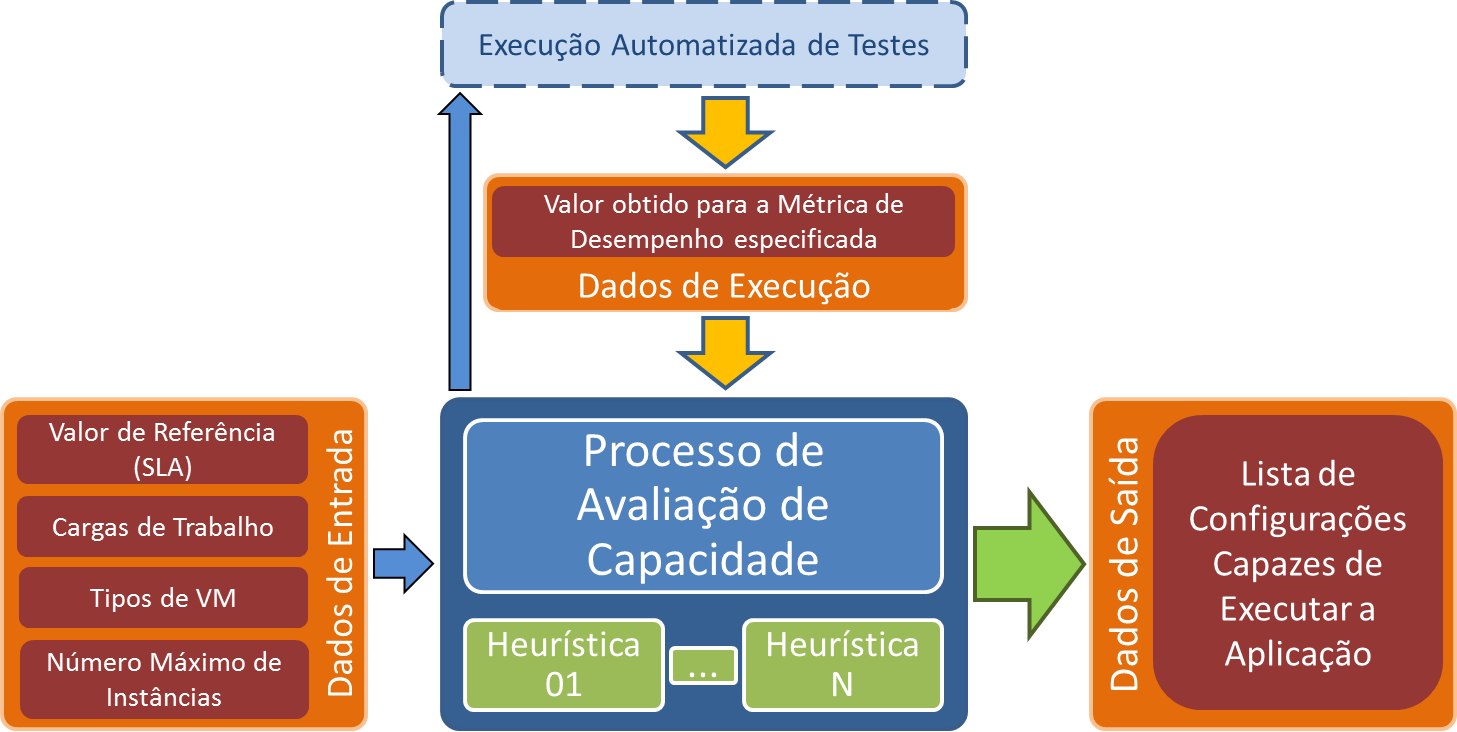
\includegraphics[trim = 20mm 5mm 20mm 5mm, scale=0.4]{img/processoAltoNivel}
%  \end{center}
%  \caption{\label{fig:fig_processo_alto_nivel}Visão geral do processo de  avaliação de capacidade.}
%\end{figure}

%O restante desta seção aborda em detalhes todas as etapas do processo proposto, explicando quais são os dados recebidos como entrada, as diferentes atividades executadas e as decisões a serem tomadas para que o processo possa determinar as configurações que atendem os requisitos de desempenho e carga de trabalho da aplicação.

\subsection{Input Data}

O principal dado de entrada esperado pelo processo é o valor de referência (SLA), o qual será usado para determinar 
se a aplicação atingiu os requisitos mínimos de desempenho exigidos em cada cenário de execução. Além do SLA, o processo precisa também conhecer quais são as cargas de trabalho sob as quais o desempenho da aplicação deverá ser avaliado. Outro dado importante que deve ser passado como entrada para o processo é o espaço de implantação da aplicação. Para isso, o processo deve ser alimentado com três parâmetros: (i) uma lista de tipos de máquinas virtuais fornecidos pelo provedor no qual deseja-se hospedar a aplicação; (ii) a quantidade máxima de máquinas virtuais de cada tipo que irá compor cada configuração a ser avaliada; e (iii) um ou mais critérios para estabelecimento das relações de capacidade entre as configurações do espaço de implantação. A Seção~\ref{sec:experiments} ilustra alguns critérios que podem ser usados para este fim. 

%Para dar um exemplo de como os três parâmetros acima são utilizados na construção do espaço de implantação, considere que o processo recebeu um único tipo de máquina virtual; o valor 3 como sendo a quantidade máxima de máquinas virtuais por configuração; e a quantidade de máquinas virtuais de cada configuração como critério para estabelecimento das relações de capacidade. Nesse caso, o espaço de implantação seria composto por 3 configurações distintas, contendo 1, 2 e 3 máquinas do tipo passado como parâmetro, respectivamente. Além disso, configurações maiores (ou seja, contendo um maior número de máquinas virtuais) seriam classificadas acima de configurações menores na hierarquia de níveis de capacidade estabelecida sobre o espaço de implantação.


A Figura~\ref{fig_niveis_capacidade} mostra um pequeno exemplo de um espaço de implantação, no qual 6 configurações,
pertencentes a duas categorias distintas, foram classificadas em dois níveis de capacidade dentro de cada categoria. Nesse exemplo, os retângulos representam as configurações, com o rótulo de cada retângulo indicando o tipo e a quantidade de máquinas virtuais que compõem a configuração, e as setas que ligam as configurações representam a existência de uma relação de capacidade elas. A ausência de seta entre duas configurações implica a impossibilidade de se estabelecer uma relação de capacidade entre elas. 

(... explicar melhor as configurações do exemplo e como foram definidas as suas relações de capacidade!)

\begin{figure}[t]
  \begin{center}
    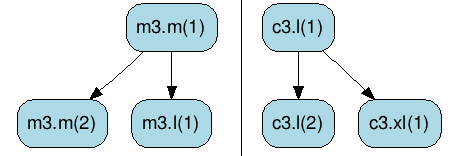
\includegraphics[scale=.5]{img/exemplo-niveis-capacidade}
  \end{center}
  \caption{\label{fig_niveis_capacidade}Exemplo de relações e níveis de capacidade entre configurações.}
\end{figure}



\subsection{Process Activities}

\begin{figure}[t]
  \centering
    %trim option's parameter order: left bottom right top
    %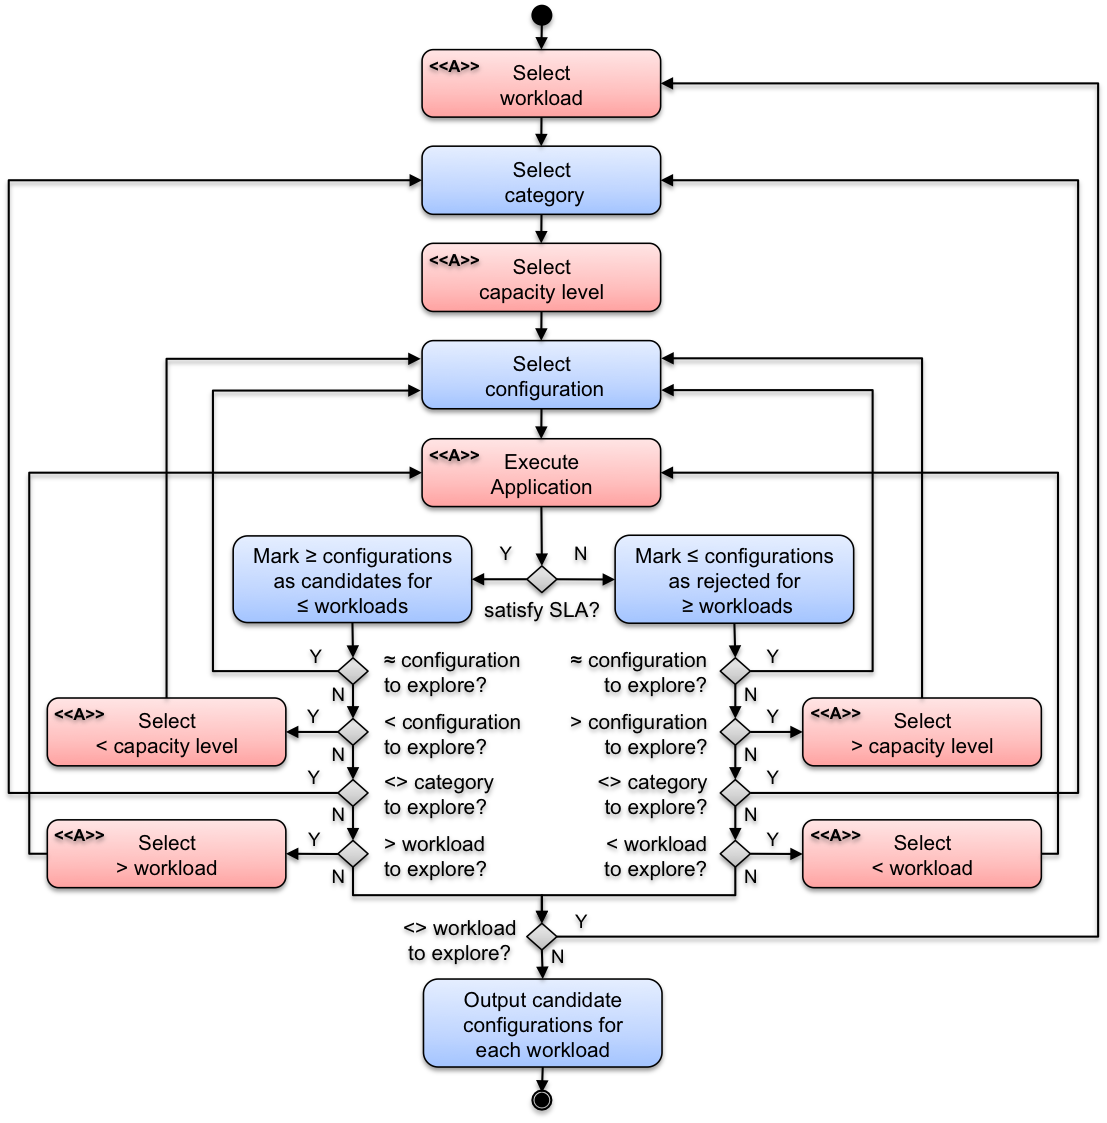
\includegraphics[trim = 0mm 0mm 0mm 0mm, scale=.5]{img/capacity-planning-diagram-v13-1-color-eng}
    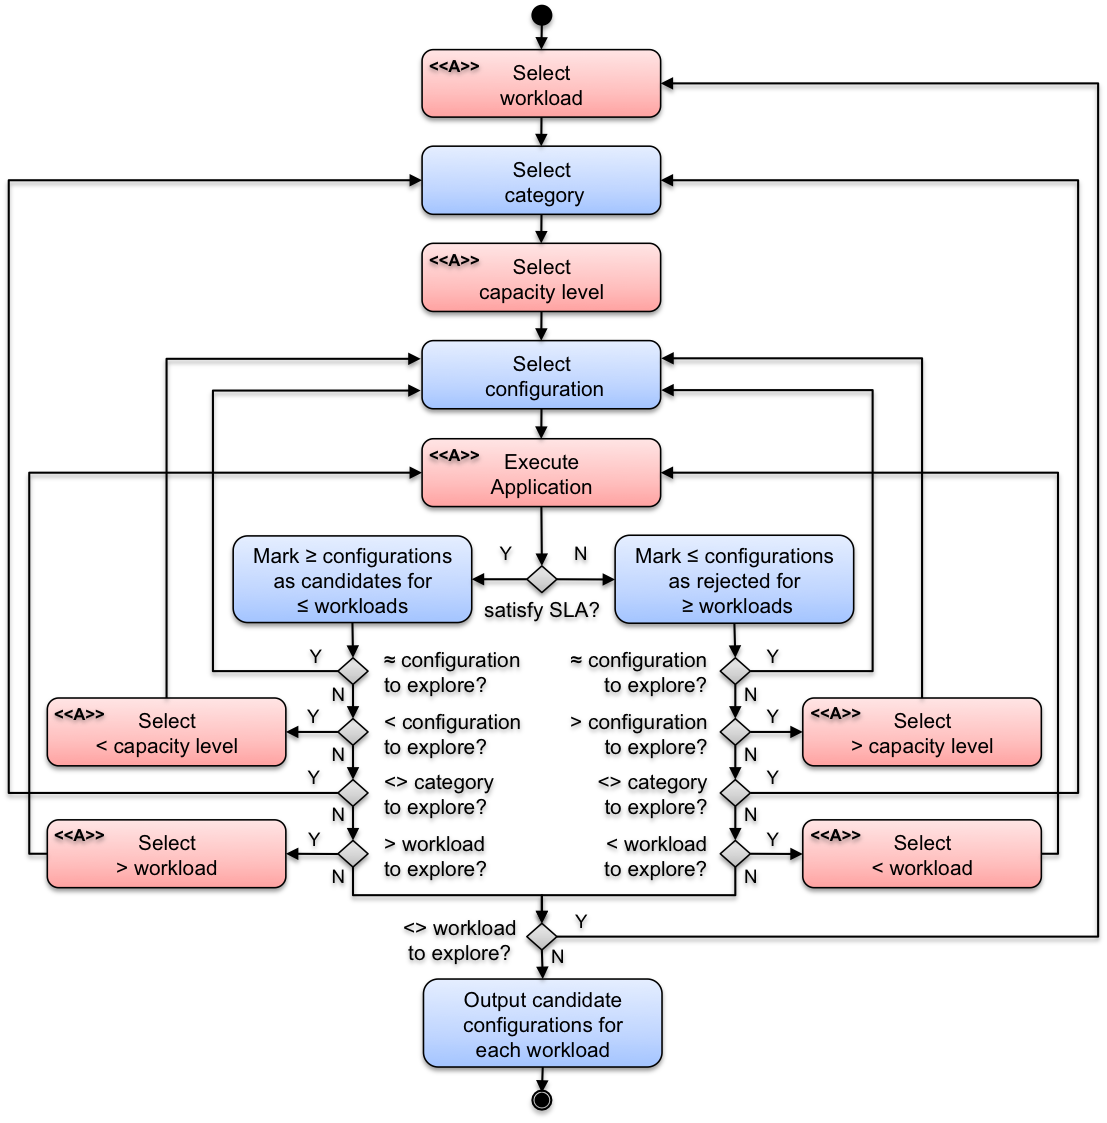
\includegraphics[width=\columnwidth]{img/capacity-planning-diagram-v13-1-color-eng}
\caption{\label{fig:process}Diagrama de atividades do processo de avaliação de capacidade.}
\end{figure}


As principais atividades executadas pelo processo de avaliação de capacidade são ilustradas no diagrama da Figura~\ref{fig:process}. As atividades destacas com o rótulo \mbox{\scriptsize\boldmath$\ll${\sc a}$\gg$} são atividades abstratas, devendo ser customizadas pelos usuários do processo de acordo com diferentes estratégias de avaliação (descritas na Seção~\ref{sec:strategies}). As outras atividades são executadas de maneira idêntica independentemente de qual seja a aplicação sob teste ou de qual seja a estratégia de avaliação utilizada. 

A execução do processo acontece em quatro fases bem distintas e cíclicas: seleção do cenário de execução da aplicação; execução da aplicação; inferência de desempenho; e seleção do próximo cenário. Cada uma dessas fases será detalhada a seguir.


\subsubsection{Selection of an Initial Execution Scenario}

A primeira atividade dessa fase é a escolha de uma carga de trabalho. Essa é uma atividade abstrata, significando que 
diferentes estratégias podem ser empregadas nessa escolha, por exemplo,
selecionando um carga de trabalho maior ou menor dentre aquelas fornecidas como dados de entrada ao processo. Depois de selecionar a carga inicial, o processo seleciona uma categoria de máquinas virtuais. No caso da categoria, a ordem ou método utilizado na escolha é irrelevante para o processo, uma vez que todas as categorias do espaço de implantação deverão ser avaliadas. Em seguida, o processo seleciona um nível de capacidade dentre aqueles presentes no espaço de implantação. Essa também é uma atividade abstrata, uma vez que níveis de capacidade mais acima ou mais abaixo na hierarquia podem ser escolhidos, a depender da estratégia de avaliação utilizada. Por fim, o processo seleciona uma configuração do nível de capacidade previamente selecionado. A ordem de seleção das configurações também é irrelevante, uma vez que todas as configurações daquele nível de capacidade devem ser avaliadas. 

\subsubsection{Application Execution}

Uma vez escolhidos uma carga de trabalho, uma categoria, um nível de capacidade e uma configuração, o processo está apto a executar a aplicação na nuvem. A execução da aplicação também é uma atividade abstrata do processo, pois depende de uma série de fatores que são específicos de cada aplicação ou plataforma de nuvem, como as tecnologias necessárias parar implantar os componentes da aplicação na nuvem bem como para submetê-los aos níveis de carga de trabalho desejados.  Após a execução da aplicação, o processo analisa o resultado obtido e passa para a fase de inferência de desempenho.

\subsubsection{Performance Inference}

Nesta fase, o processo se bifurca, atingindo seu primeiro ponto de decisão. A partir da análise do resultado da execução, que é feita comparando-se os indicadores obtidos para a métrica de desempenho utilizada frente ao valor de referência (SLA) desejado, o processo determina se a aplicação é ou não capaz de atender à demanda imposta sobre ela com a atual configuração. Se a aplicação satisfaz o SLA, o processo assinala a configuração atual como uma {\em configuração candidata} para o atual nível de carga. Do contrário, o processo assinala a configuração atual como uma {\em configuração rejeitada} para esse nível de carga.

É neste momento que a abordagem de inferência de desempenho, proposta originalmente neste trabalho, entra em ação. Com base nas relações de capacidade presentes no espaço de implantação, o processo pode ``inferir'' o provável desempenho da aplicação para outras configurações e cargas de trabalho ainda não avaliadas. Ora, se o processo identificou que uma certa configuração consegue satisfazer a demanda imposta à aplicação sob uma certa carga de trabalho, intuitivamente qualquer outra configuração de maior poder computacional também será capaz de fazê-lo sob a mesma carga de trabalho. Similarmente, é intuitivo concluir que a mesma configuração também será capaz de satisfazer o SLA da aplicação sob cargas de trabalho menores. Assim, usando as informações sobre as relações de capacidade existentes entre as configurações do espaço de implantação, o processo também assinala como candidatas para o atual nível de carga todas as outras configurações identificadas como sendo de ``maior capacidade'' que a configuração atual de acordo com o espaço de implantação. Da mesma forma, o processo também assinala a configuração atual como candidata para todos os níveis de carga inferiores ao nível de carga atual.

O caso em que a configuração atual não satisfaz o SLA  da aplicação é tratado de modo análogo. Nesse caso, o processo assinala como rejeitadas para o atual nível de carga todas as outras configurações identificadas como sendo de ``menor capacidade'' que a configuração atual de acordo com o espaço de implantação. O mesmo acontece com a configuração atual, que também é assinalada como rejeitada para todos os outros níveis de carga superiores ao nível de carga atual.


O efeito da inferência de desempenho pode ser melhor visualizado através do exemplo de espaço de implantação mostrado na Figura~\ref{fig:fig_processo_inferencia}. Nesse exemplo, o espaço de implantação está representado na forma de uma matriz, cujas linhas correspondem às configurações e as colunas correspondem às cargas de trabalho. Note que o nível de capacidade das configurações cresce de cima para baixo na matriz, enquanto o tamanho da carga de trabalho cresce da esquerda para a direita. A parte inferior esquerda da matriz ilustra o caso em que o SLA é satisfeito em um determinado cenário de execução. Já a parte superior direita ilustra o caso oposto. As células marcadas com um ``{\scriptsize \raisebox{0.4ex}{\boldmath$\surd{}\,$}}'' (``\boldmath$\times{}$'') indicam as configurações marcadas como candidatas (rejeitadas) para as respectivas cargas de trabalho. As duas células em destaque correspondem a execuções reais da aplicação, cujos resultados serviram de base para a inferência do desempenho da aplicação nos outros cenários. 


\begin{figure}[t]
  \begin{center}
    %trim option's parameter order: left bottom right top
    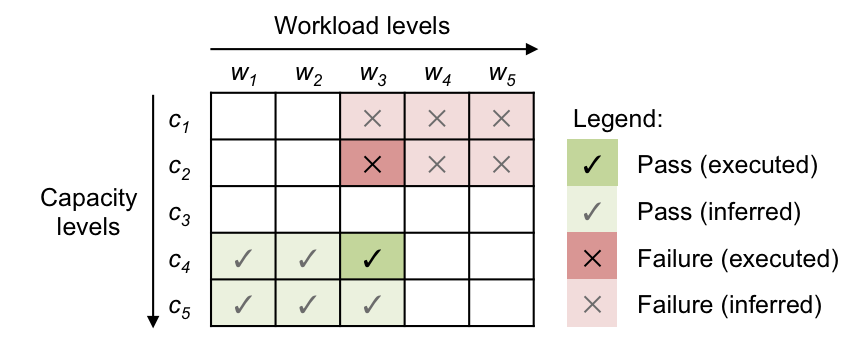
\includegraphics[trim = 0mm 0mm 0mm 0mm, scale=.55]{img/inference}
  \end{center}
  \caption{\label{fig:fig_processo_inferencia}Ilustração da marcação de configurações como {\em candidatas} (embaixo à esquerda) ou {\em rejeitadas} (no alto à direita) via inferência de desempenho.}
\end{figure}


Esse exemplo é representativo do grande potencial da abordagem de inferência de desempenho para reduzir os custos associados ao processo de planejamento de capacidade, tonando-o mais rápido e eficiente. Note que, considerando os dois casos ilustrados, o processo teria obtido resultados relativos à avaliação de 12 cenários de execução distintos, dos quais apenas dois teriam de fato sido executados na nuvem, o que representa uma economia de quase 90\% em relação à abordagem empírica tradicional, onde todos os cenários de interesse devem ser sistematicamente avaliados.

Na seção~\ref{sec:experiments}, apresentaremos resultados obtidos empiricamente mostrando que a abordagem de inferência de desempenho consegue prever o desempenho esperado de uma aplicação na nuvem com alta precisão. 

\subsubsection{Selection of the Next Execution Scenario}

Após a fase de inferência de desempenho, o processo seleciona os elementos que comporão o próximo cenário de execução a ser avaliado, ou encerra sua execução, caso não haja mais cenários a explorar. Nesse caso, o processo produz, como saída, uma lista contendo todas as configurações assinaladas como candidatas para cada carga de trabalho avaliada, em ordem crescente de preço.

A seleção do próximo cenário inclui a escolha de uma nova configuração do atual nível de capacidade, a escolha de um novo nível de capacidade (que deverá ser maior ou menor que o nível de capacidade atual, a depender do resultado da execução da aplicação no atual cenário), a escolha de uma nova categoria, ou a escolha de uma nova carga de trabalho (que também deverá ser maior ou menor que o nível de carga atual, novamente a depender do resultado da execução da aplicação no atual cenário). As escolhas do novo nível de capacidade e da nova carga de trabalho também são atividades abstratas, a serem definidas de acordo com a estratégia de avaliação utilizada para customizar o processo. 


\subsection{Evaluation Strategies}\label{sec:strategies}

Conforme mencionado anteriormente, todas as atividades abstratas do processo (com exceção da atividade de execução da aplicação na nuvem) devem ser customizadas de acordo com diferentes estratégias de avaliação. Essas atividades incluem, basicamente, a escolha de cargas de trabalho e níveis de capacidade. Tais escolhas influenciam diretamente a maneira através da qual o processo explora o espaço de implantação, tendo um forte impacto no alcance da inferência de desempenho. 

Como exemplo, considere o caso de um espaço de implantação onde nenhuma configuração é capaz de atender a 
demanda da aplicação sob qualquer nível de carga. Nesse caso, iniciar o processo de avaliação pelas 
configurações do nível de capacidade mais baixo sob cargas de trabalho maiores não seria uma boa estratégia, 
uma vez que o número de configurações e cargas de trabalho para os quais o desempenho esperado da 
aplicação poderia ser inferido seria muito pequeno. Por outro lado, iniciar o processo pelas configurações de nível 
de capacidade mais alto sob cargas de trabalho menores seria um estratégia muito melhor, já que assim seria possível 
inferir o desempenho da aplicação para praticamente todas as outras
configurações e todas as outras cargas de trabalho, representando uma grande economia de tempo e custo.

Esses dois extremos ilustram bem o desafio de se escolher os cenários de execução mais promissores do ponto de vista da inferência de desempenho. A fim de enfrentar esse desafio, este trabalho introduz o conceito das {\em heurísticas de seleção}, que agregam táticas a serem observadas no momento em que o processo, via alguma estratégia de avaliação, precisa escolher uma nova configuração ou uma nova carga de trabalho para compor um novo cenário de execução. Nesse sentido, foi inicialmente definido um conjunto de três táticas de seleção, denominadas {\em otimista}, {\em conservadora} e {\em pessimista}, respectivamente, aplicáveis tanto à escolha de novas cargas de trabalho quanto à escolha de novos níveis de capacidade. A combinação dessas três táticas na escolha de novos cenários de execução dá origem a nove heurísticas de seleção, ilustradas na Figura~\ref{fig:heuristicas}.


\begin{figure}[t]
  \begin{center}
    %trim option's parameter order: left bottom right top
    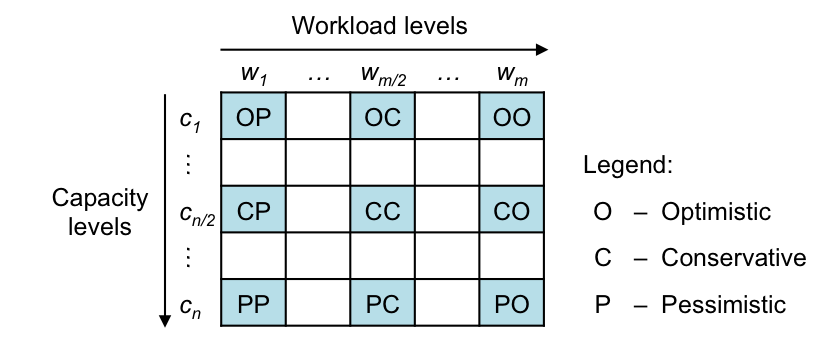
\includegraphics[trim = 0mm 0mm 0mm 0mm, scale=.55]{img/heuristics2}
  \end{center}
  %\caption{\label{fig:heuristicas}Heurísticas de seleção utilizadas no processo de avaliação de capacidade.}
  \caption{\label{fig:heuristicas}Heurísticas para seleção de configurações e cargas de trabalho.}
\end{figure}


Nessa figura, as heurísticas são identificadas por diferentes pares de letras posicionados ao longo da matriz que representa o espaço de implantação. A primeira letra que identifica a heurística refere-se à tática usada na escolha da configuração (linha), enquanto a segunda letra refere-se à tática usada na escolha da carga de trabalho (coluna). Como pode-se observar, a tática otimista leva à escolha de configurações menores e cargas de trabalho maiores. Já a tática conservadora leva à escolha de configurações e cargas de trabalho de nível intermediário. Por fim, a tática pessimista leva à escolha de configurações maiores e cargas de trabalho menores.
 
 
 
No contexto do processo de avaliação de capacidade proposto neste trabalho, cada heurística de seleção fornece uma ``lógica'' diferente para exploração do espaço de implantação, servindo como base para a customização do processo com diferentes estratégias de avaliação. A acurácia e a eficiência do processo proposto, em particular, da abordagem de inferência de desempenho, utilizando cada uma das noves heurísticas de seleção mencionas acima, serão analisadas na próxima seção. 

%\subsection{Example}

%\subsection{Implementation}

\section{Experimental Evaluation}\label{sec:experiments}

Esta seção descreve o experimento realizado como forma de verificação do processo de avaliação de capacidade apresentado anteriormente. Inicialmente, é apresentada a metodologia utilizada para a condução do experimento. Em seguida, são apresentados os resultados obtidos por cada uma das nove heurísticas de seleção propostas. Esses resultados são usados tanto para uma comparação qualitativa das heurísticas entre si, quanto para atestar
a eficiência do processo proposto e de sua abordagem de inferência de desempenho. 

É importante mencionar que o processo proposto foi implementado e está disponível na forma de uma ferramenta web,\footnote{\scriptsize \url{http://cloud-capacitor.herokuapp.com/}.} a qual foi utilizada para executar o experimento descrito a seguir. Devido a restrições de espaço, os detalhes da implementação do processo bem como de sua ferramenta de apoio estão fora do escopo deste artigo.

\subsection{Method}

O experimento consistiu na realização de sessões de avaliação de
capacidade de uma aplicação web real (WordPress,\footnote{\scriptsize \url{https://wordpress.org/}.} escolhida por ser uma das aplicações de criação e administração de \emph{blogs} mais utilizadas atualmente) implantada em um provedor de nuvem também real (Amazon EC2,\footnote{\scriptsize \url{http://aws.amazon.com/ec2}.} escolhido por ser o líder de mercado entre provedores IaaS públicos). O WordPress foi implantado em duas camadas: uma para o banco de  dados MySQL, e outra para o servidor de aplicação, executada pelo servidor Apache HTTPD. Como balanceador de carga, foi utilizada uma máquina dedicada executando o servidor web Nginx. 


% A aplicação escolhida foi o WordPress \cite{wordpress}, um motor de construção 
% e administração de \emph{blogs}. Sua escolha foi motivada por ser uma aplicação
% bem conhecida, de utilização via web, ideal para implantação em ambiente de
% nuvem, e com componentes arquiteturais escaláveis. Além disso, o fluxo de 
% utilização típico da aplicação apresenta características bem diversificadas quanto ao uso
% de recursos de CPU e memória, rede, sistema de arquivos e banco de dados.

Devido a restrições de custo e tempo, o experimento limitou-se a variar 
apenas a camada de aplicação, usando de 1 a 4 servidores Apache executando o WordPress. 
A execução dos testes foi orquestrada pelo ambiente Cloud~Crawler~\cite{cunha2013b},
que automatizou as tarefas de iniciar e parar todas as instâncias de máquinas virtuais, configurar 
o balanceador de carga de acordo com o número de instâncias testadas na camada de 
aplicação, iniciar e parar a execução dos testes, gerar as cargas de trabalho impostas à aplicação e, finalmente, coletar os dados de desempenho obtidos em cada teste. A Figura~\ref{fig:implantacao} mostra um panorama dessa arquitetura de implantação.

\begin{figure}[t]
  \begin{center}
    %trim option's parameter order: left bottom right top
    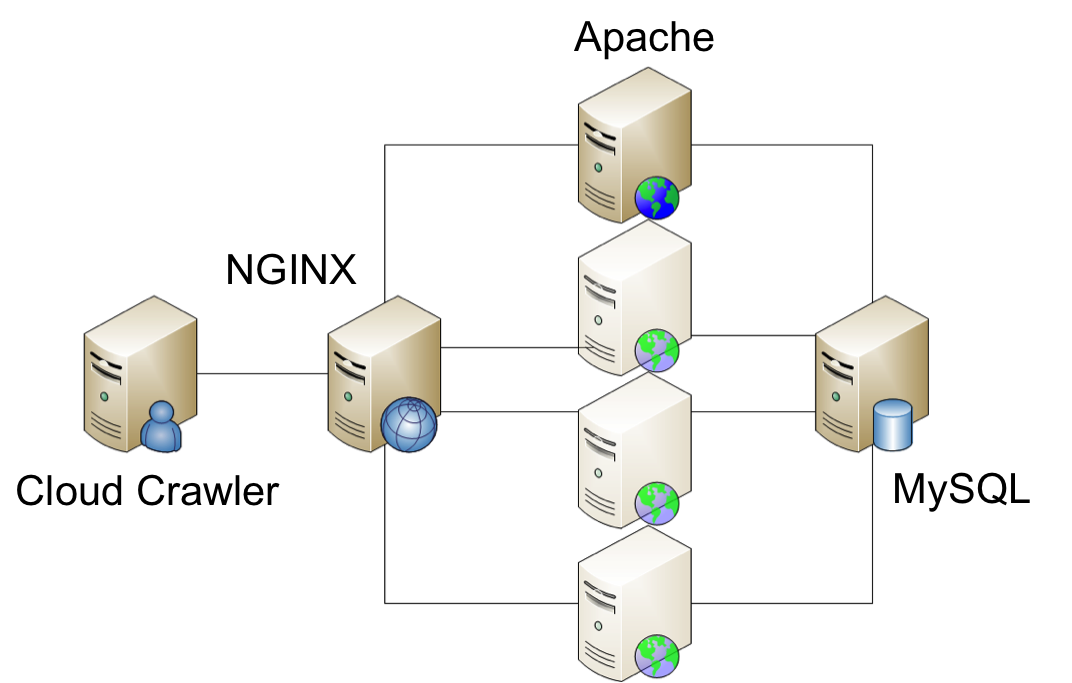
\includegraphics[trim = 0mm 0mm 0mm 0mm, scale=0.35]{img/WordPress-deployment}
  \end{center}
  \caption{\label{fig:implantacao}Arquitetura de implantação do WordPress na Amazon EC2.}
\end{figure}


Para compor o espaço de implantação utilizado no experimento, 
foram escolhidos sete tipos de máquinas virtuais oferecidos pelo provedor Amazon EC2:
{\em m3\_medium}, {\em m3\_large}, {\em m3\_xlarge}, {\em m3\_2xlarge}, {\em c3\_large}, {\em c3\_xlarge} e {\em c3\_2xlarge}. Para cada um desses tipos, foram criadas configurações
com 1, 2, 3 e 4 instâncias, levando a um total de 28 configurações diferentes no espaço de implantação, divididas em duas categorias distintas, ``m3'' e ``c3''. As relações de capacidade entre essas configurações foram definidas separadamente, para cada categoria, de modo a refletir o tipo e a quantidade de máquinas virtuais presentes em cada configuração. Assim, configurações com um certo número de máquinas virtuais de um determinado tipo eram consideradas de capacidade superior (inferior) a outras configurações contendo máquinas do mesmo tipo em menor (maior) quantidade. De maneira similar, configurações contendo o um certo número de máquinas virtuais de um certo tipo eram consideradas de capacidade superior (inferior) a outras configurações com a mesma quantidade de máquinas mas de tipos diferentes se estes tipos fossem inferiores (superiores) ao tipo da primeira configuração, de acordo com a classificação dos tipos definidas pelo próprio provedor de nuvem.  Por exemplo, a configuração composta por 3 máquinas to tipo {\em m3\_2xlarge} era considerada superior a outra configuração composta por apenas 2 máquinas deste mesmo tipo. Da mesma forma, a configuração formada por 2 máquinas do tipo  {\em c3\_large} era considerada inferior a outra configuração com a mesma quantidade de máquinas do tipo {\em c3\_xlarge}.

As cargas de trabalho utilizadas no experimento foram quantificadas em número de usuários concorrentes enviando requisições ao WordPress. Foi definido um total de 10 cargas de trabalho, representando 100, 200, 300, 400, 500, 600, 700, 800, 900 e 1000 usuários concorrentes, respectivamente. 

De forma a estabelecer uma \emph{baseline} para comparação da eficiência e da acurácia do processo proposto, especificamente de suas diferentes heurísticas de seleção, foram coletados dados de desempenho do WordPress na nuvem para cada um dos 280 cenários possíveis, ou seja, foram efetivamente realizados testes de desempenho da aplicação para cada uma das 28 configurações criadas sob cada uma das 10 cargas de trabalho especificadas. Esse conjunto
de dados de execuções reais da aplicação foi denominado {\em oráculo}, e a estratégia necessária para gerar todos esses dados foi denominada heurística {\em Força Bruta} (em Inglês, {\em Brute Force -- BF}). As nove heurísticas propostas foram então comparadas entre si e com a heurística BF.

Cada teste de desempenho consistiu em executar o WordPress utilizando uma das 28 configurações definidas para o espaço de implantação e então submetê-lo a uma das 10 cargas de trabalho especificadas durante um período de 1 hora. Durante os testes, um gerador de carga criava a quantidade de usuários corresponde à carga de trabalho sendo avaliada. Cada usuário realizava a seguinte sequência de requisições à aplicação: efetuar \emph{logon}; inserir uma nova postagem; consultar a nova postagem; alterar a nova postagem; consultar postagens existentes por palavra-chave; alterar uma postagem existente; e, finalmente, efetuar \emph{logoff}. 

A métrica de desempenho utilizada no experimento foi o {\em tempo de resposta total}, ou 
seja, o tempo total decorrido entre o envio da primeira requisição da sequência 
acima e o momento em que o usuário recebeu a resposta para última requisição da
sequência. Assim, para ser considerada como candidata para uma determinada carga de trabalho, uma configuração devia ser capaz de atender, sem erros, pelo menos  90\% das sequências de requisições recebidas dos usuários da aplicação em um tempo total igual ou inferior ao valor do SLA, tal como definido no respectivo parâmetro de entrada do processo.

\subsection{Results}

\subsubsection{Efficiency}
Esta subseção apresenta os resultados de eficiência atingidos pelas heurísticas
de seleção usadas no processo sob dois aspectos distintos: o custo total da avaliação e a quantidade de execuções realizadas por cada heurística. Esse custo foi calculado somando-se o preço da hora de utilização, conforme a tabela de preços do provedor na data realização dos testes, para cada uma das configurações para as quais foram realizadas execuções reais na nuvem. 

A Figura~\ref{fig:cost-time} mostra os gráficos dos resultados obtidos pelas
nove heurísticas em relação a essas duas métricas, considerando SLAs 
de 10, 20, 30, 40 e 50 segundos. No topo de cada gráfico vê-se uma linha horizontal
escura que representa os resultados da heurística BF. Note que, como essa heurística não efetua nenhuma inferência quanto ao desempenho da aplicação, seus resultados, tanto em termos de custo quanto em termos de número de execuções, são sempre constantes, independente do SLA requerido.

%\begin{figure}[t]
%\centering%\footnotesize
%  %trim option's parameter order: left bottom right top
%  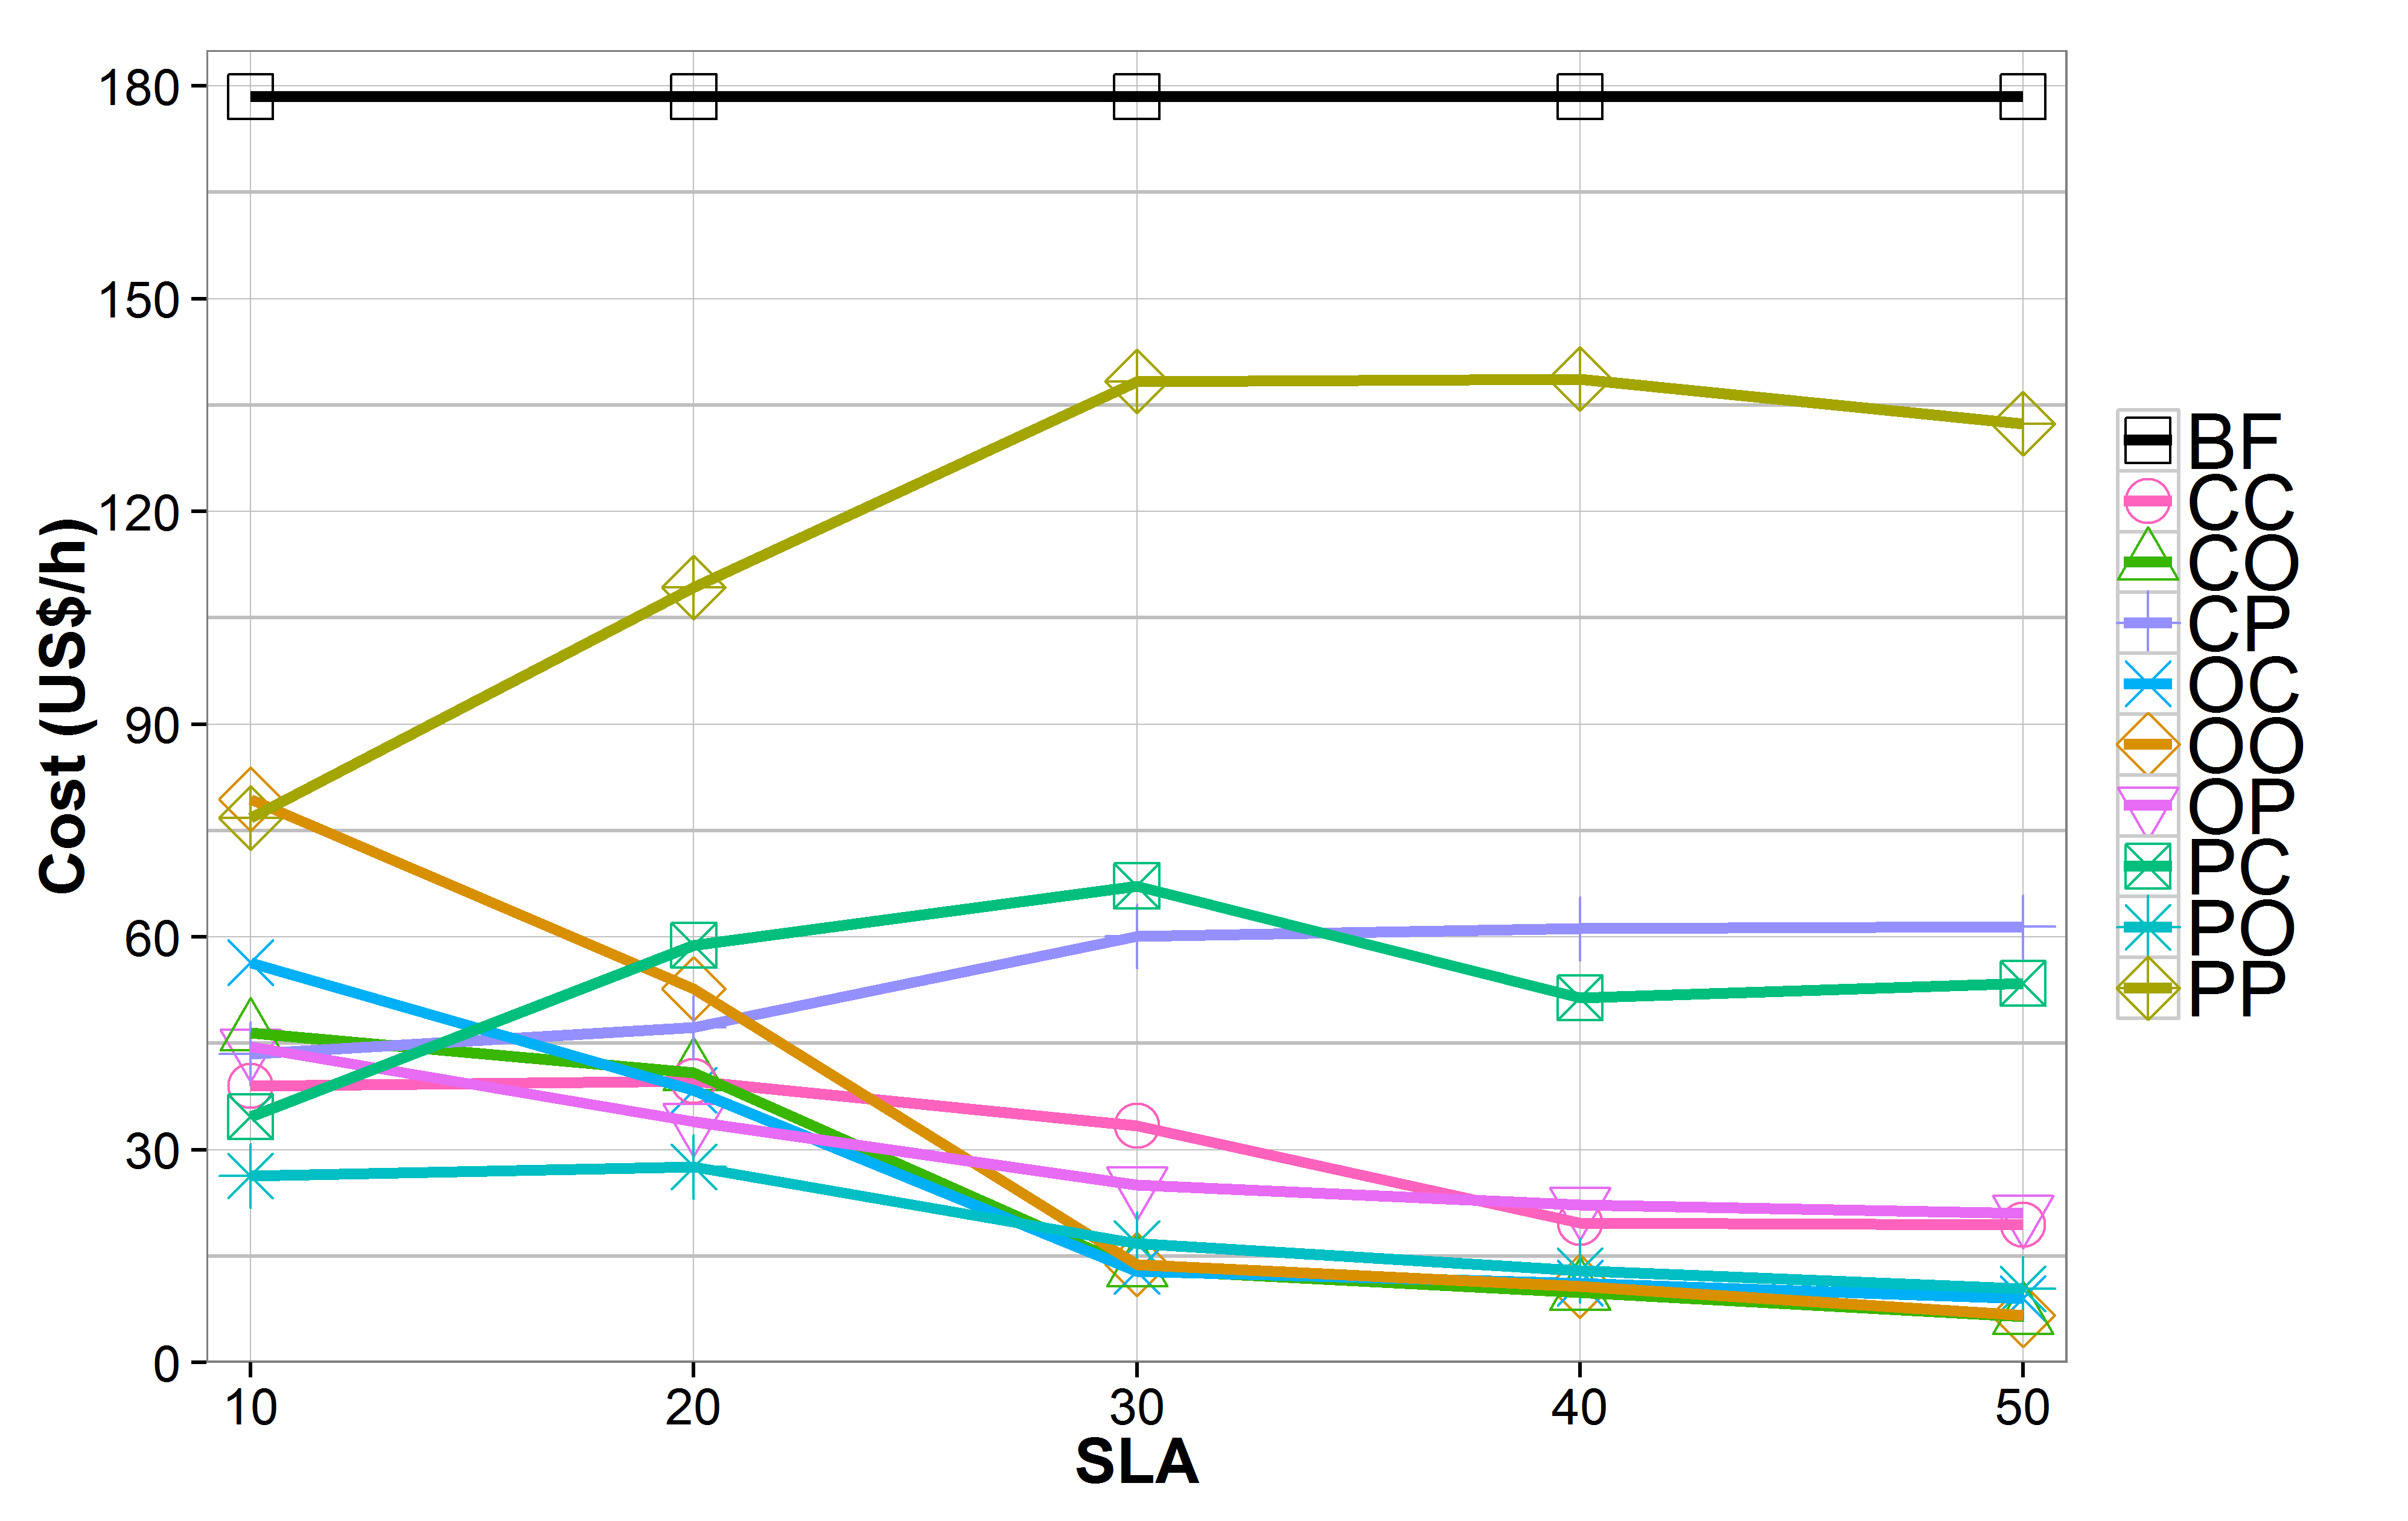
\includegraphics[trim = 0mm 0mm 0mm 0mm, width=.85\columnwidth]{img/graphic-cost-capacity.png}\\(a)\\
%  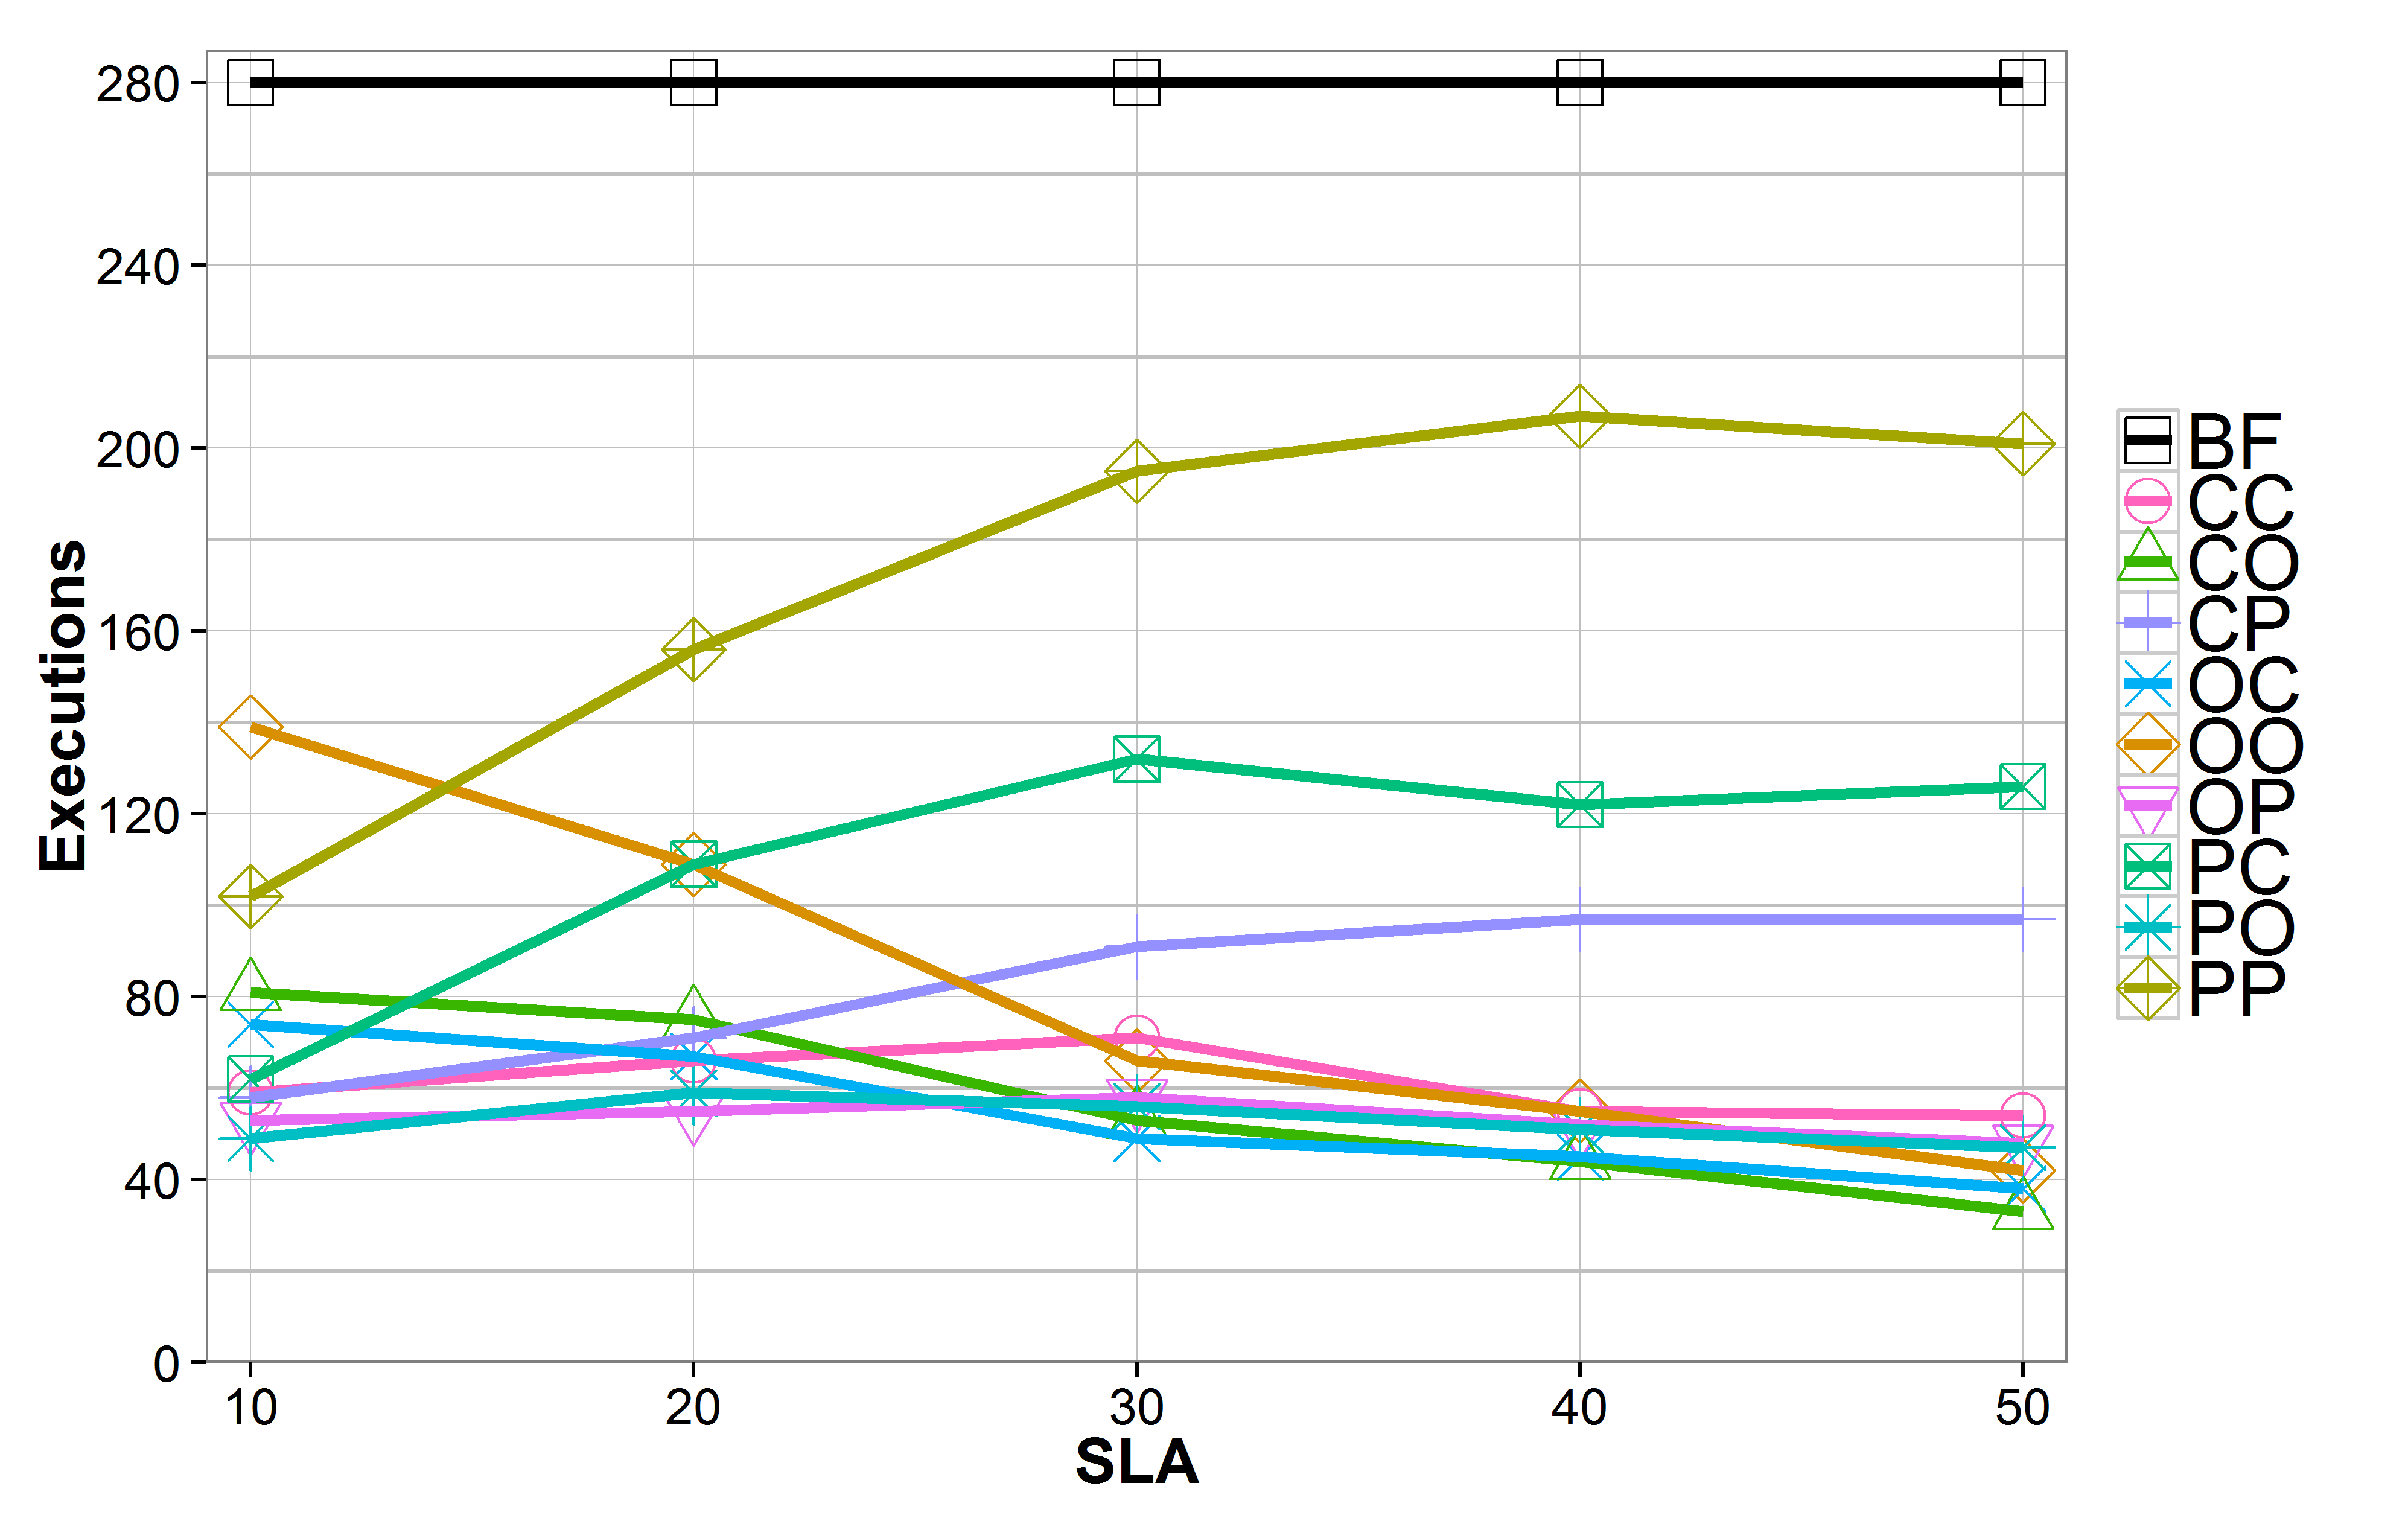
\includegraphics[trim = 0mm 0mm 0mm 0mm, width=.95\columnwidth]{img/graphic-time-capacity.png}\\(b)
%  \caption{\label{fig:cost-time}Eficiência das heurísticas de seleção: (a) custo e (b) execuções.}
%\end{figure}

\begin{figure}[!t]
\centering
\subfloat[]{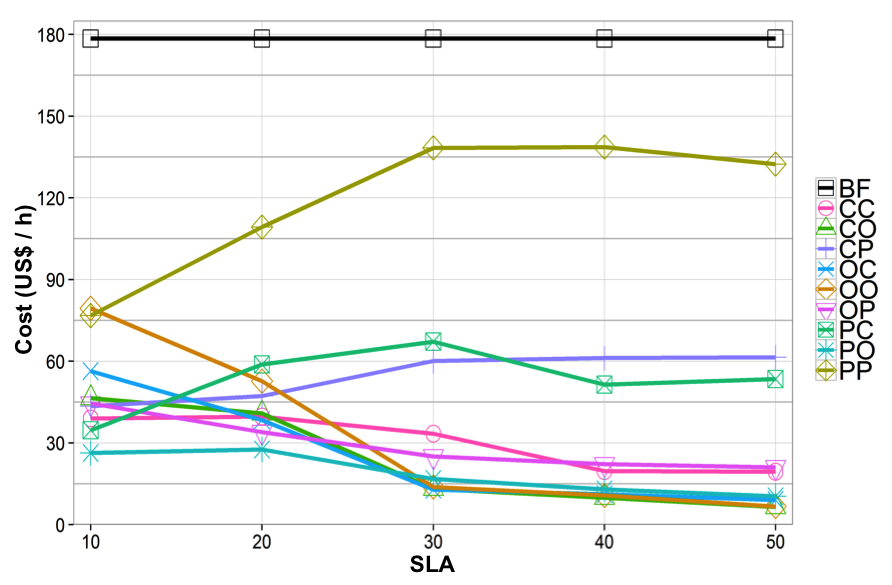
\includegraphics[width=.8\columnwidth]{img/graphic-cost-capacity2.png}%
\label{fig:cost}}
%\hfil
\\
\subfloat[]{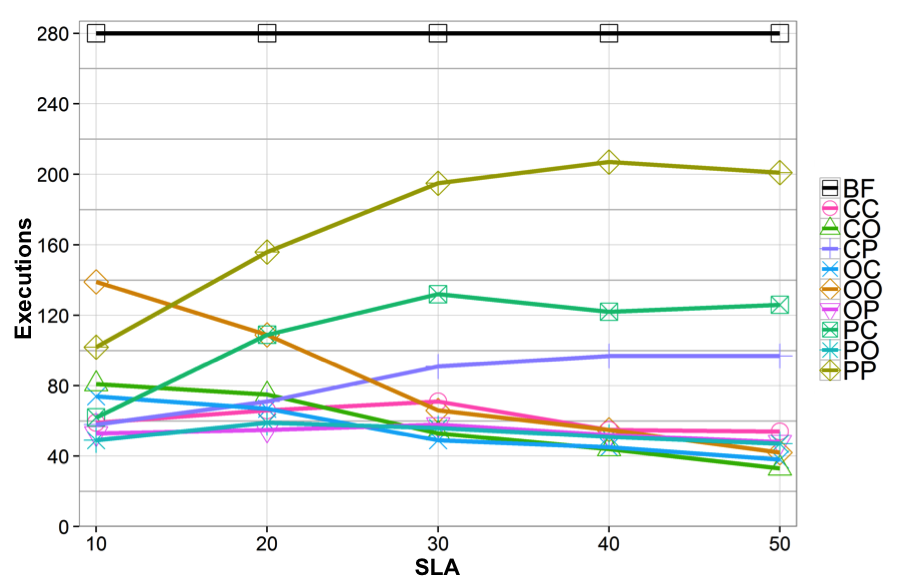
\includegraphics[width=.8\columnwidth]{img/graphic-time-capacity2.png}%
\label{fig:time}}
\caption{Eficiência das heurísticas de seleção: (a) custo e (b) execuções.}
\label{fig:cost-time}
\end{figure}

(... melhorar e expandir análise dos resultados!)

A análise do gráfico de custo (Figura~\ref{fig:cost}) mostra que mesmo a heurística com o pior desempenho no que se refere ao custo já apresenta uma redução considerável 
em relação à heurística BF. Por outro lado, as melhores heurísticas chegam a 
representar uma economia da ordem de 96\% em comparação com o que seria gasto
com a execução de todas as combinações de configurações e cargas de trabalho.
Embora o comportamento das heurísticas varie em função do SLA, é possível notar
que quando a exigência do SLA é mais moderada, o comportamento de todas as heurísticas
se estabiliza, tornando possível identificar que algumas delas tendem a
ser mais econômicas que as outras. Ainda que não seja possível afirmar que uma só 
heurística seja a melhor em todas as situações, pode-se considerar que a heurística
Pessimista/Otimista (PO) se mostra como a mais econômica em geral. A heurística
Conservadora/Otimista (CO) merece atenção para os SLAs mais brandos, com os menores
custos absolutos nessas circunstâncias. 

A análise do gráfico de execuções reais na nuvem (Figura~\ref{fig:time}), por sua vez, mostra uma redução de até 88\% em relação aos resultados da heurística BF. Os menores números de execuções são atingidos pelas heurísticas Otimista/Conservadora (OC) e Conservadora/Otimista (CO), sob os SLAs mais brandos. Porém, como não se saem tão 
bem sob SLAs mais rígidos, como 10 segundos, a heurística PO ganha destaque por ter comportamento mais estável, figurando entre as mais econômicas no aspecto de quantidade de execuções sob a maioria dos SLAs avaliados. 

Vale ressaltar que a significativa redução do número de execuções necessárias durante o processo de planejamento de capacidade, decorrente da utilização da abordagem de inferência de desempenho, conforme mostrado nesta seção, implica não apenas em economia de tempo e horas de máquinas para os usuários da nuvem, mas também pode contribuir de forma decisiva para a reduzir outros tipos de custo típicos de qualquer projeto, como esforço e alocação de recursos humanos .

%\begin{figure}[t]
%  \begin{center}
%    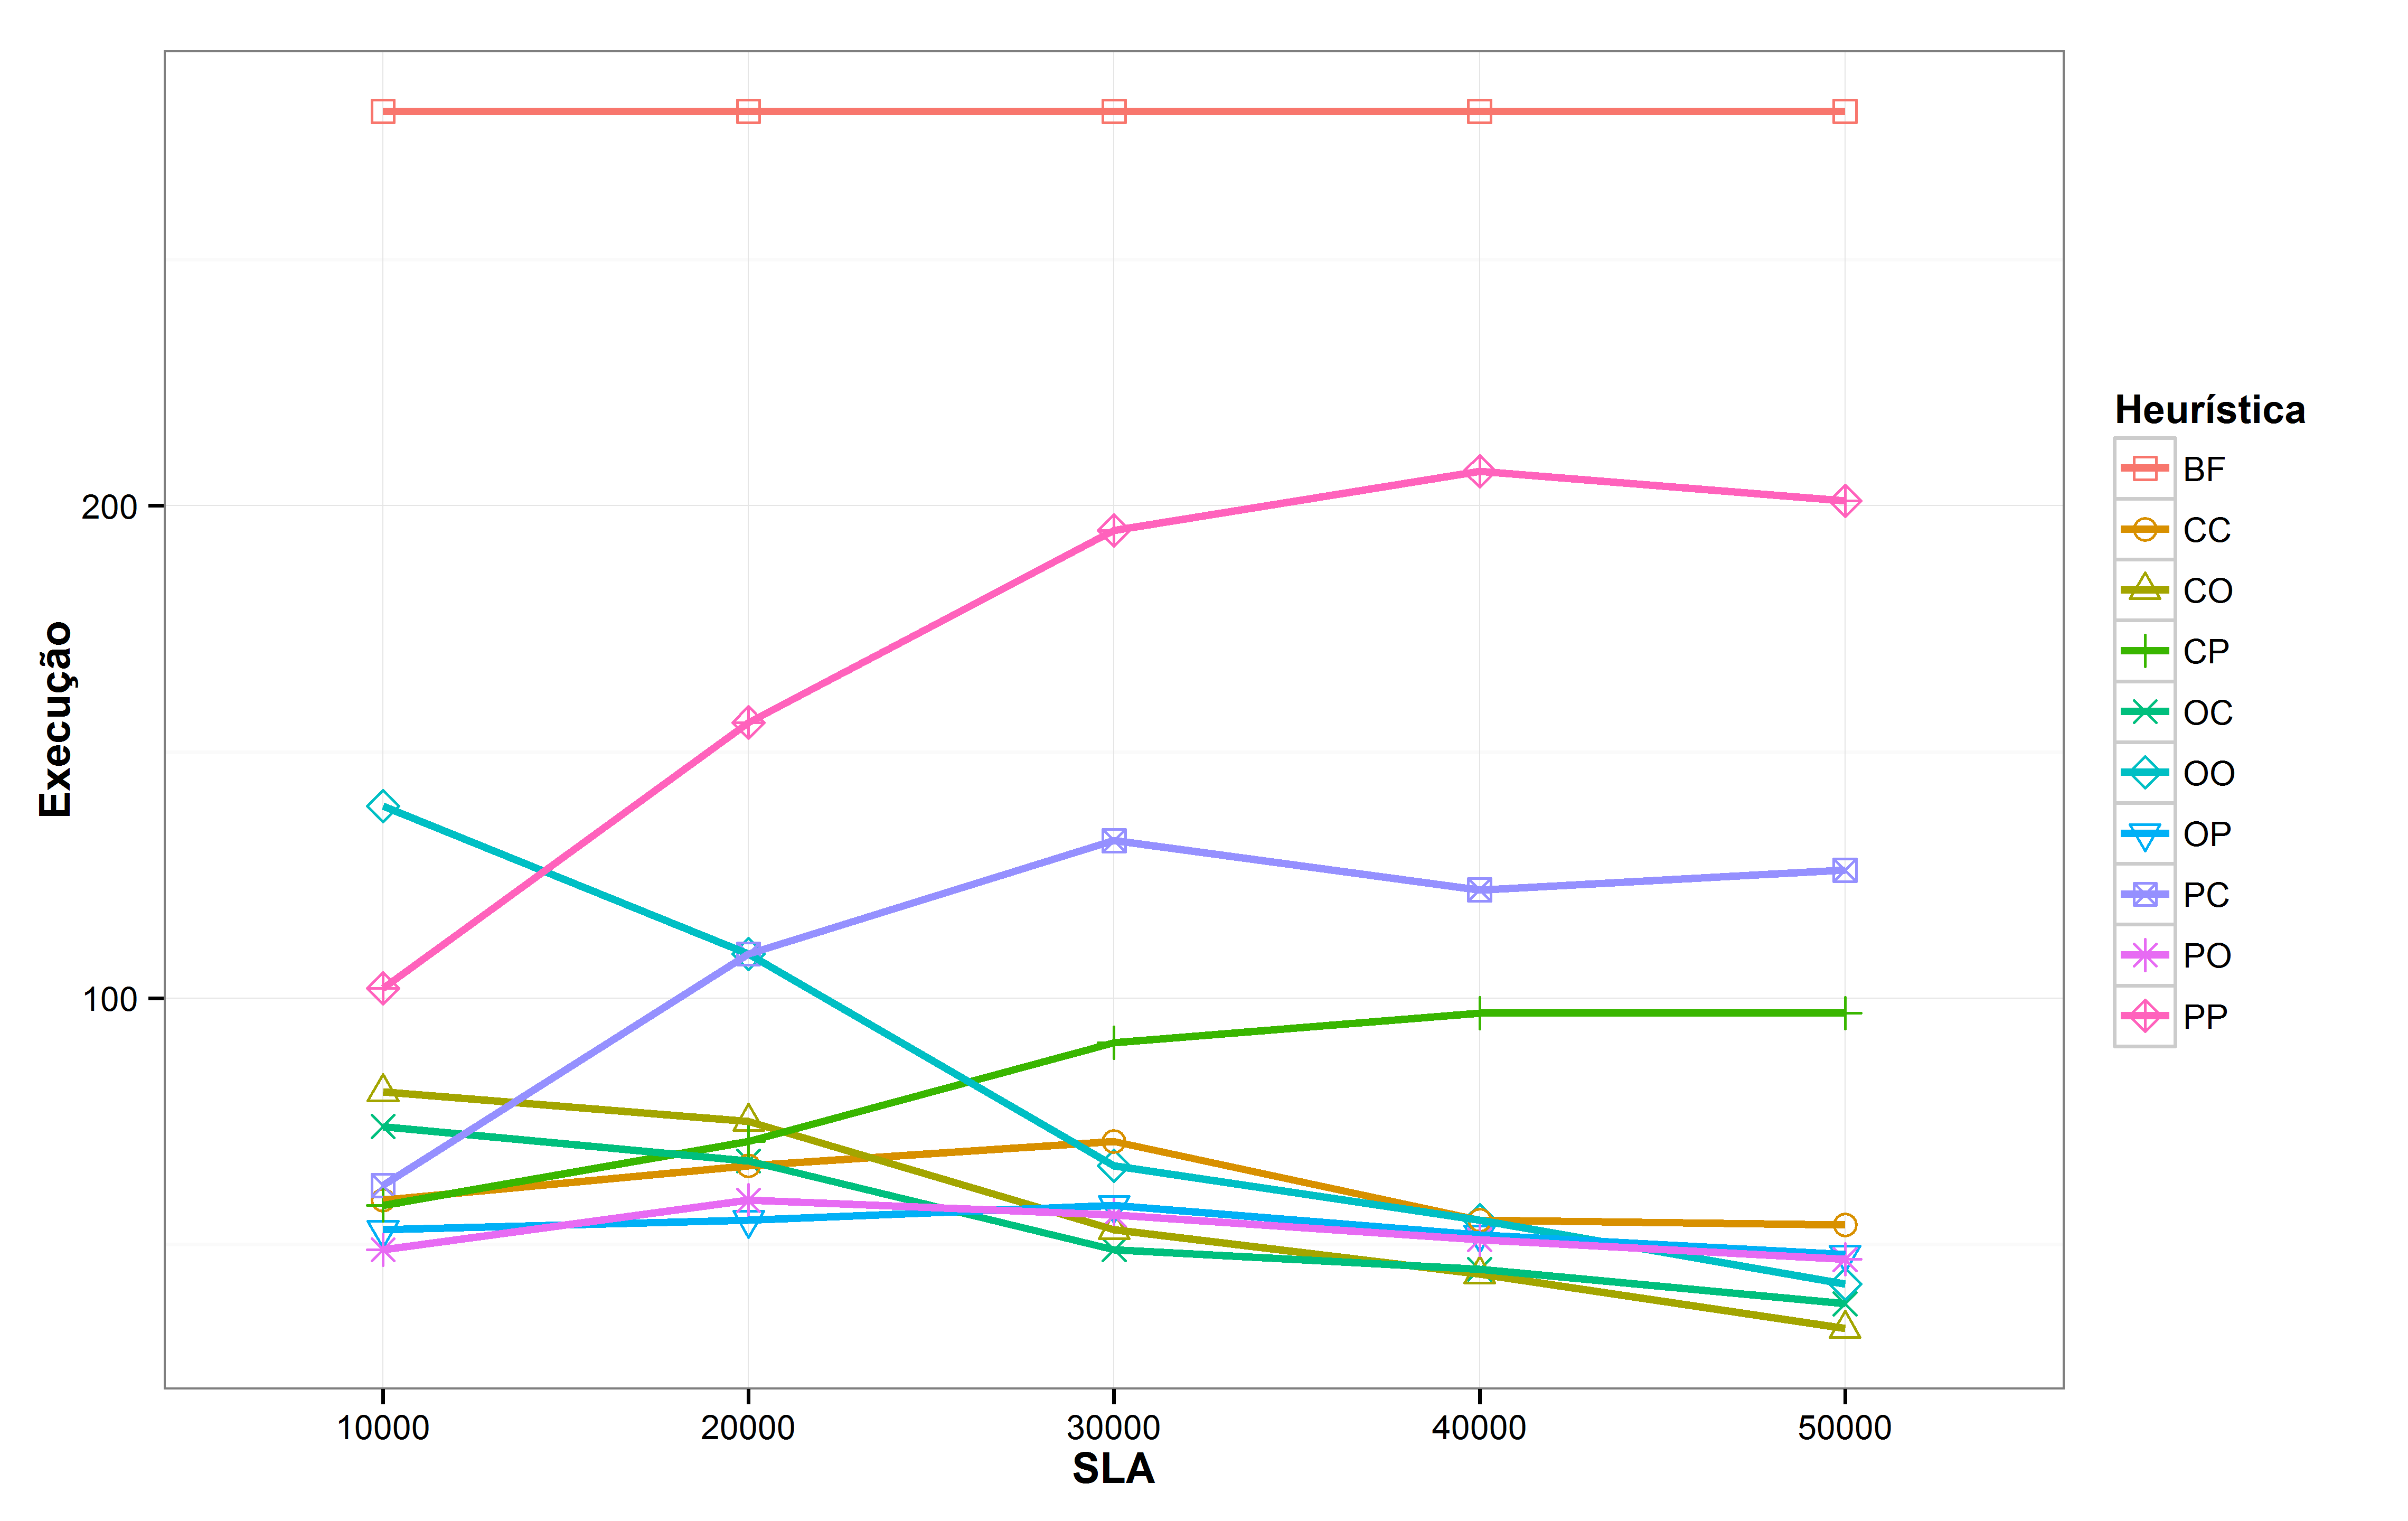
\includegraphics[scale=0.3]{img/ExecutionCount-Capacity}
%  \end{center}
%  \caption{\label{fig:eficiencia_execucoes}Avaliação da Eficiência do Número de Execuções das Heurísticas.}
%\end{figure}

%Tanto no aspecto custo como no aspecto quantidade de execuções, nota-se que a heurística Pessimista/Pessimista (PP) tem um desempenho bem inferior às demais heurísticas, exigindo um número de execuções significativamente maior e, por isso, resultam em maiores tempo e custo para o processo de planejamento de capacidade. As heurísticas Pessimista/Conservadora (PC) e Conservadora/Pessimista (CP) ainda aparecem um pouco descoladas do desempenho das outras heurísticas, embora com uma redução em torno de 65\% no número de execuções.



\subsubsection{Accuracy}

\unboldmath

Para medir a acurácia do processo de avaliação de capacidade, foram calculados os valores médios de \emph{Precision}, \emph{Recall} e \emph{F-Measure}~\cite{Baeza-Yates1999} para os resultados produzidos por cada uma das heurísticas de seleção sob os diferentes valores de SLA avaliados, tomando como base os dados do oráculo.  

(... explicar as três métricas!)

Para isso, os dados do oráculo foram utilizados para determinar se as configurações identificadas como candidatas (resultados positivos) e rejeitadas (resultados negativos) por cada heurística para uma determinada carga de trabalho eram de fato verdadeiras (nesse caso, as predições teriam sido corretas) ou falsas (nesse caso, as predições teriam sido erradas).

Sejam $TP(w,s)$, $FP(w,s)$ e $FN(w,s)$ os resultados positivos verdadeiros, resultados positivos falsos e resultados negativos falsos, respectivamente, obtidos por uma heurística de seleção $h$ sob uma carga de trabalho $w$ e um SLA $s$. Os valores de \emph{Precision}, \emph{Recall} e \emph{F-Measure} para a heurística $h$ sob a carga de trabalho $w$ e SLA $s$, denotados por $P(h,w,s)$, $R(h,w,s)$ e $F(h,w,s)$, respectivamente, são calculados pelas seguintes fórmulas~\cite{Baeza-Yates1999}:

{\scriptsize
  %
  $P(h,w,s) = \dfrac{TP(h,w,s)}{TP(h,w,s)\,+\,FP(h,w,s)}$
  
 \smallskip
  %
 $R(h,w,s) = \dfrac{TP(h,w,s)}{TP(h,w,s)\,+\,FN(h,w,s)}$
 
 \smallskip
   %
  $F(h,w,s) = 2\,\times\,\dfrac{P(h,w,s)\,\times\,R(h,w,s)}{P(h,w,s)\,+\,R(h,w,s)}$
  }

Considerando $m$ cargas de trabalho (denotadas por $w_{1}$, $w_{2}$,\,$\ldots$\,, $w_{m}$), as fórmulas para o cálculo das médias dessas três métricas para uma heurística $h$ e SLA $s$,  denotados por $P(h,s)$, $R(h,s)$ e $F(h,s)$, respectivamente, são as seguintes: 

{\scriptsize
$P(h,s) = \sum\limits_{i=1}^{m}\,P(h,w_{i},s)\,/\,m$

\smallskip
%
$R(h,s) = \sum\limits_{i=1}^{m}\,R(h,w_{i},s)\,/\,m$

\smallskip
%
$F(h,s) = \sum\limits_{i=1}^{m}\,F(h,w_{i},s)\,/\,m$
}


A Tabela~\ref{tab:accuracy} mostra os valores de $P$, $R$ e $F$ calculados para as nove heurísticas de seleção sob os cinco níveis de SLA investigados no experimento. Nota-se que em apenas um dos cinco SLAs o processo deixou de obter 100\% de acurácia nas predições, apresentando uma taxa de erro inferior a 3\% para $P$ e $R$, e de aproximadamente 1\% para $F$.  


\begin{table}[t]
\setlength{\tabcolsep}{1.2pt}
   \centering%\scriptsize
   \caption{\label{tab:accuracy}Accuracy of the proposed selection heuristics.}
    %\begin{tabular}{m{.9cm}*{5}{m{.2em}m{.2em}m{.4em}}}
    %\begin{tabular}{*{16}{c}}
    \begin{tabular}{|c|*{5}{ccc|}}
    \hline
    %\toprule
     \multirow{3}{*}{Heuristic} & \multicolumn{15}{c|}{SLA} \\
    \cline{2-16}
            & \multicolumn{3}{c|}{10} & \multicolumn{3}{c|}{20} & \multicolumn{3}{c|}{30} & \multicolumn{3}{c|}{40} & \multicolumn{3}{c|}{50} \\
          \cline{2-16}
             & $P$     & $R$     & $F$     & $P$     & $R$     & $F$     & $P$     & $R$     & $F$     & $P$     & $R$  & $F$     & $P$     & $R$     & $F$ \\%[-.3cm]
          \hline
          %\midrule          
    CC    & 1.00  & 1.00  & 1.00  & 1.00  & 1.00  & 1.00  & 1.00  & \textcolor{red}{0.98}  & \textcolor{red}{0.99}  & 1.00  & 1.00  & 1.00  & 1.00  & 1.00  & 1.00 \\
    CO    & 1.00  & 1.00  & 1.00  & 1.00  & 1.00  & 1.00  & \textcolor{red}{0.99}  & 1.00  & \textcolor{red}{0.99}  & 1.00  & 1.00  & 1.00  & 1.00  & 1.00  & 1.00 \\
    CP    & 1.00  & 1.00  & 1.00  & 1.00  & 1.00  & 1.00  & 1.00  & \textcolor{red}{0.98}  & \textcolor{red}{0.99}  & 1.00  & 1.00  & 1.00  & 1.00  & 1.00  & 1.00 \\
    OC    & 1.00  & 1.00  & 1.00  & 1.00  & 1.00  & 1.00  & \textcolor{red}{0.99}  & \textcolor{red}{0.99}  & \textcolor{red}{0.99}  & 1.00  & 1.00  & 1.00  & 1.00  & 1.00  & 1.00 \\
    OO    & 1.00  & 1.00  & 1.00  & 1.00  & 1.00  & 1.00  & \textcolor{red}{0.99}  & 1.00  & \textcolor{red}{0.99}  & 1.00  & 1.00  & 1.00  & 1.00  & 1.00  & 1.00 \\
    OP    & 1.00  & 1.00  & 1.00  & 1.00  & 1.00  & 1.00  & 1.00  & \textcolor{red}{0.98}  & \textcolor{red}{0.99}  & 1.00  & 1.00  & 1.00  & 1.00  & 1.00  & 1.00 \\
    PC    & 1.00  & 1.00  & 1.00  & 1.00  & 1.00  & 1.00  & 1.00  & \textcolor{red}{0.98}  & \textcolor{red}{0.99}  & 1.00  & 1.00  & 1.00  & 1.00  & 1.00  & 1.00 \\
    PO    & 1.00  & 1.00  & 1.00  & 1.00  & 1.00  & 1.00  & \textcolor{red}{0.99}  & 1.00  & \textcolor{red}{0.99}  & 1.00  & 1.00  & 1.00  & 1.00  & 1.00  & 1.00 \\
    PP    & 1.00  & 1.00  & 1.00  & 1.00  & 1.00  & 1.00  & 1.00  & \textcolor{red}{0.98}  & \textcolor{red}{0.99}  & 1.00  & 1.00  & 1.00  & 1.00  & 1.00  & 1.00 \\
    \hline
    %\toprule
    \end{tabular}%
 \end{table}%

Uma investigação mais minuciosa dos dados de desempenho da aplicação na nuvem revelou que essa pequena perda na qualidade das predições foi devida a flutuações ocasionais no desempenho de alguns dos tipos de máquinas virtuais disponibilizadas pelo provedor. Essas flutuações levaram algumas das configurações avaliadas a terem um desempenho superior ao de outras configurações consideradas de maior capacidade de acordo com o espaço de implantação. (... detalhar quais configurações causaram o problema!)

Tais flutuações afetaram particularmente o desempenho da aplicação para o SLA de 30 segundos, refletindo em erros de predição. De fato, oscilações no desempenho da infraestrutura virtualizada oferecida por provedores de nuvem IaaS são relativamente comuns, como observados por \cite{iosup2011performance} e \cite{cunha2011investigating}. O impacto dessas flutuações nos resultados observados no experimento, porém, foi mínimo (afetando um único nível de SLA com taxa de erro médio de 1\%), o que reforça a confiança de que a abordagem de inferência de desempenho proposta neste trabalho pode atingir alta acurácia mesmo para aplicações e plataformas de nuvem reais.  


\section{Related Work}\label{sec:related-work}

Esta seção analisa várias soluções existentes para apoiar os usuários de nuvens IaaS no planejamento da capacidade necessária às suas aplicações. Conforme mencionado previamente, essas soluções seguem duas abordagens principais, aqui denominadas de preditiva e empírica. 

%Na abordagem preditiva, a
%aplicação alvo não é executada diretamente no ambiente onde se deseja implantá-la,~\cite{cloudharmony},~\cite{malkowski2010cloudxplor,li2011,jung2013cloudadvisor,fittkau2012cdosim} e~\cite{li2011cloudprophet}, fazem uso dessa abordagem. Já em~\cite{jayasinghe2012,silva2013cloudbench,cunhacloud} e~\cite{scheuner2014cloud} são apresentados trabalhos que utilizam a abordagem empírica, onde as aplicações alvo são implantadas na nuvem e então
%submetidas a testes de carga.

As soluções da abordagem preditiva utilizam diferentes técnicas de predição do desempenho da aplicação, com destaque para a analogia com os resultados obtidos através da execução de diversos {\em benchmarks} na nuvem, normalmente coletados {\em a priori} pelo provedor da solução~\cite{malkowski2010cloudxplor,cloudharmony,li2011,jung2013cloudadvisor}; simulação do comportamento esperado da aplicação através de um simulador de nuvem~\cite{fittkau2012cdosim}; e reprodução na nuvem de eventos relevantes do ponto de vista de desempenho, como utilização de CPU, memória e disco, capturados a partir da execução local da aplicação~\cite{li2011cloudprophet}. Embora de baixo custo (com
exceção da solução descrita em~\cite{li2011cloudprophet}, que necessita adquirir recursos da nuvem para reproduzir os eventos da aplicação) e, no caso de soluções que suportam predições por analogia, de baixa complexidade, esses trabalhos ainda deixam a desejar em termos de acurácia, devido a limitações importantes das técnicas de predição adotadas. Mais especificamente, a predição por analogia tem pouco eficácia se os {\em bechmarks} disponíveis não possuem perfis de comportamento similares ao da aplicação sob teste. Já os simuladores de nuvem ainda não conseguem atingir um nível de fidelidade próximo ao comportamento real de uma aplicação implantada em um provedor de nuvem público, chegando a apresentar diferenças de desempenho superiores a 30\%~\cite{fittkau2012cdosim}. Um problema similar ocorre com a solução que reproduz eventos da aplicação na nuvem, cujo mecanismo de captura de eventos ainda possui sérias limitações de ordem prática~\cite{li2011cloudprophet}.

As soluções empíricas, por outro lado, oferecem alta acurácia na avaliação do desempenho da aplicação na nuvem, uma vez que são baseadas em dados de desempenho obtidos diretamente no provedor~\cite{jayasinghe2012,silva2013cloudbench,cunha2013b,scheuner2014cloud}. Além disso, essas soluções são muito mais flexíveis, no sentido em que permitem aos usuários avaliar diferentes combinações de componentes da aplicação sob as mais variadas configurações de recursos e cargas de trabalho. O ponto negativo das soluções que adotam a abordagem empírica é a necessidade de executar cada um dos cenários definidos pelo usuário, uma vez que elas não oferecem nenhum mecanismo voltado especificamente para reduzir a quantidade de execuções da aplicação. Dessa forma, cabe exclusivamente aos usuários dessas soluções definirem as melhores estratégias de explorar o espaço de implantação da aplicação na nuvem.

Nesse contexto, o novo processo de avaliação de capacidade apresentado neste trabalho segue uma abordagem híbrida, combinando aspectos positivos das abordagens preditiva e empírica. Em contraste às soluções da abordagem preditiva, o novo processo realiza predições com base em relações de capacidade definidas entras diferentes configurações de recursos de um mesmo provedor de nuvem, e em resultados empíricos obtidos a partir da execução da própria aplicação neste provedor. Com isso, o novo processo consegue alta acurácia nas predições ao mesmo que reduz significativamente a quantidade de cenários de implantação que precisam ser efetivamente testados na nuvem. 


% An example of a floating figure using the graphicx package.
% Note that \label must occur AFTER (or within) \caption.
% For figures, \caption should occur after the \includegraphics.
% Note that IEEEtran v1.7 and later has special internal code that
% is designed to preserve the operation of \label within \caption
% even when the captionsoff option is in effect. However, because
% of issues like this, it may be the safest practice to put all your
% \label just after \caption rather than within \caption{}.
%
% Reminder: the "draftcls" or "draftclsnofoot", not "draft", class
% option should be used if it is desired that the figures are to be
% displayed while in draft mode.
%
%\begin{figure}[!t]
%\centering
%\includegraphics[width=2.5in]{myfigure}
% where an .eps filename suffix will be assumed under latex, 
% and a .pdf suffix will be assumed for pdflatex; or what has been declared
% via \DeclareGraphicsExtensions.
%\caption{Simulation Results}
%\label{fig_sim}
%\end{figure}

% Note that IEEE typically puts floats only at the top, even when this
% results in a large percentage of a column being occupied by floats.


% An example of a double column floating figure using two subfigures.
% (The subfig.sty package must be loaded for this to work.)
% The subfigure \label commands are set within each subfloat command, the
% \label for the overall figure must come after \caption.
% \hfil must be used as a separator to get equal spacing.
% The subfigure.sty package works much the same way, except \subfigure is
% used instead of \subfloat.
%
%\begin{figure*}[!t]
%\centerline{\subfloat[Case I]\includegraphics[width=2.5in]{subfigcase1}%
%\label{fig_first_case}}
%\hfil
%\subfloat[Case II]{\includegraphics[width=2.5in]{subfigcase2}%
%\label{fig_second_case}}}
%\caption{Simulation results}
%\label{fig_sim}
%\end{figure*}
%
% Note that often IEEE papers with subfigures do not employ subfigure
% captions (using the optional argument to \subfloat), but instead will
% reference/describe all of them (a), (b), etc., within the main caption.


% An example of a floating table. Note that, for IEEE style tables, the 
% \caption command should come BEFORE the table. Table text will default to
% \footnotesize as IEEE normally uses this smaller font for tables.
% The \label must come after \caption as always.
%
%\begin{table}[!t]
%% increase table row spacing, adjust to taste
%\renewcommand{\arraystretch}{1.3}
% if using array.sty, it might be a good idea to tweak the value of
% \extrarowheight as needed to properly center the text within the cells
%\caption{An Example of a Table}
%\label{table_example}
%\centering
%% Some packages, such as MDW tools, offer better commands for making tables
%% than the plain LaTeX2e tabular which is used here.
%\begin{tabular}{|c||c|}
%\hline
%One & Two\\
%\hline
%Three & Four\\
%\hline
%\end{tabular}
%\end{table}


% Note that IEEE does not put floats in the very first column - or typically
% anywhere on the first page for that matter. Also, in-text middle ("here")
% positioning is not used. Most IEEE journals/conferences use top floats
% exclusively. Note that, LaTeX2e, unlike IEEE journals/conferences, places
% footnotes above bottom floats. This can be corrected via the \fnbelowfloat
% command of the stfloats package.

\section{Conclusion and Future Work}\label{sec:conclusion}

A tarefa de escolher adequadamente os recursos computacionais (ex.: máquinas
virtuais) de um provedor de nuvem, de forma a minimizar os custos necessários para atender diferentes níveis de demanda de uma aplicação, é um desafio importante para o qual ainda não existem soluções plenamente satisfatórias disponíveis. Este trabalho apresentou um novo processo de avaliação de capacidade por inferência de desempenho, que se mostrou uma solução ao mesmo tempo eficiente (em termos de custo e tempo) e eficaz (em termos da acurácia dos resultados) para apoiar a planejar a capacidade de aplicações na nuvem. 

%Resultados preliminares, obtidos a partir da implantação de uma aplicação real (WordPress) em um popular provedor de nuvem público (Amazon EC2), mostraram que o processo consegue reduções significativas de custo e tempo, de até 96\% e 86\%, respectivamente, em relação a abordagem empírica tradicional, identificando as melhores configurações de recursos para a aplicação alvo com acurácia média próxima a 99\%.

Com relação aos trabalhos futuros, algumas possibilidades interessantes para melhoria ou extensão deste trabalho incluem: realizar novos experimentos visando investigar se os resultados reportados neste artigo são generalizáveis para outras aplicações e provedores de nuvem; investigar de novas heurísticas de seleção de configurações e cargas de trabalho, que levem em conta dados sobre a utilização dos recursos da nuvem pela aplicação, como consumo de CPU e memória; e propor novos critérios para definir as relações de capacidade entre as diferentes configurações disponibilizadas pelo provedor de nuvem, por exemplo, considerando o custo de cada configuração, e investigar seu impacto no desempenho das heurísticas de seleção.

% conference papers do not normally have an appendix


% use section* for acknowledgement
\section*{Acknowledgment}

%The authors would like to thank the reviewers for their insightful comments and suggestions, which greatly improved the final version of the paper. 

This work is partially supported by Brazil's National Council for Scientific and Technological Development (CNPq), under grants 311617/2011-5 and 487174/2012-7.

% trigger a \newpage just before the given reference
% number - used to balance the columns on the last page
% adjust value as needed - may need to be readjusted if
% the document is modified later
%\IEEEtriggeratref{8}
% The "triggered" command can be changed if desired:
%\IEEEtriggercmd{\enlargethispage{-5in}}

% references section

% can use a bibliography generated by BibTeX as a .bbl file
% BibTeX documentation can be easily obtained at:
% http://www.ctan.org/tex-archive/biblio/bibtex/contrib/doc/
% The IEEEtran BibTeX style support page is at:
% http://www.michaelshell.org/tex/ieeetran/bibtex/
\bibliographystyle{IEEEtran}
% argument is your BibTeX string definitions and bibliography database(s)
\bibliography{IEEEabrv,principal-capacitor}
%
% <OR> manually copy in the resultant .bbl file
% set second argument of \begin to the number of references
% (used to reserve space for the reference number labels box)
%\begin{thebibliography}{1}
%
%\bibitem{IEEEhowto:kopka}
%H.~Kopka and P.~W. Daly, \emph{A Guide to \LaTeX}, 3rd~ed.\hskip 1em plus
%  0.5em minus 0.4em\relax Harlow, England: Addison-Wesley, 1999.
%
%\end{thebibliography}




% that's all folks
\end{document}


